\chapter{Turbulent inflow conditions for large-eddy simulations of wind farms}\label{ch:turbulent_inflow}
A major challenge in turbulence-resolving simulations of spatially developing flows is the generation of unsteady and coherent turbulent inflow conditions. In the context of optimal control in wind-farm LES, proper inflow conditions should contain accurate and fully-developed turbulence in order to capture important flow mechanisms such as e.g., wake meandering, turbulent wake mixing or vortex shedding. In this chapter, we will discuss the methods for generating turbulent inflow conditions used by the optimal control simulations in later chapters. Furthermore, the chapter includes novel contributions made specifically to the field of turbulent inlet generation in the context of the current PhD research. 

The chapter is outlined as follows: Firstly, Section~\ref{sec:inflow_intro} provides context for the problem of turbulent inflow generation by reviewing literature on popular synthetic turbulence
methods and periodic Navier--Stokes based precursor methods. Furthermore, a qualitative comparison between both justifies the use of precursor methods for the optimal control purposes considered in
this thesis. Second, Section~\ref{sec:inflow_CP} details the implementation of a standard precursor method in the SP--Wind framework. Next, the chapter turns to the contributions that were made
specifically to the field of precursor inflow methods in the context of the current work: Section~\ref{sec:inflow_var} discusses a generalization of standard precursor methods to time-varying inflow
directions, and Section~\ref{sec:inflow_shifted} elaborates on a new type of \emph{shifted} periodic boundary condition for precursor simulations,
designed to eliminate spurious spanwise inhomogeneities in time averages of wall-bounded turbulent flows.
Finally, Section~\ref{sec:inflow_summary} summarizes the key aspects of this chapter. 

Parts of the contents of this chapter have been published in the following journal articles:
\begin{itemize}
	\item Munters, Meneveau \& Meyers (2016), ``Shifted periodic boundary conditions for simulations of wall-bounded turbulent flows.'' \emph{Phys Fluids} \textbf{28} (2), 025112
	\item Munters, Meneveau \& Meyers (2016), ``Turbulent inflow precursor method with time-varying direction for large-eddy simulations and applications to wind farms.'' \emph{Boundary-Layer Meteorol} \textbf{159} (2), 305 -- 328. 
\end{itemize} 

\section{Turbulent inflow conditions: background and motivation}\label{sec:inflow_intro}

	Turbulence-resolving simulations of flows in which periodic boundary conditions cannot be straightforwardly invoked, carry the non-trivial problem of generating realistic turbulent inflow conditions at an acceptable computational cost. The quality of inflow turbulence has a significant influence on flow features throughout the entire simulation domain, especially in the absence of phenomena triggering turbulence development such as large-scale flow separation, transition, or unstable stratification \citep{keylock2011method}. Comprehensive overviews of inlet conditions for LES can be found in the work of \cite{keating2004priori} and, more recently, in the work of \cite{tabor2010inlet}. \cite{shur2014synthetic} provides an updated view of these methods from the point of view of turbulence generation on RANS--LES interfaces in hybrid simulations for aeronautical applications.
	
	In the remainder of this section, the two mainstream categories for generating turbulent inflow conditions, synthetic turbulence and precursor methods, are briefly elaborated from a wind-farm LES perspective. Furthermore, a qualitative comparison between these approaches is presented. Results advocate the use of precursor inflow methods for the applications to be considered.

	\subsection{Synthetic turbulence methods}
	In this approach synthetic turbulence is generated from a chosen model, before it is added to a mean inflow profile. The level of complexity of these methods ranges from (possibly filtered) random noise \cite[see, e.g.,][]{klein2003digital,munoz2015stochastic} to advanced models matching physical spectra and moments that are assumed to evolve rapidly enough  into physically accurate turbulence. Instead of random noise, one can consider a sinusoidally varying noise term with one or a few modes only \citep{mirocha2014resolved}. Most more advanced synthetic turbulence models rely on the assumption that turbulence can be specified using only low-order or one-point statistics \citep{keating2004priori}. Moreover, they assume that mean shear and turbulence can be specified independently, even though LES studies indicate that this might lead to erroneous results \citep{park2014large,mehta2014large}. The main advantage to most synthetic turbulence models is the low computational overhead compared to the target simulation of interest.
	
	In the context of wind energy and atmospheric boundary-layer flows,  the synthetic turbulence model developed by \cite{mann1998wind} is widely used.
	The model parametrizes the spectral tensor of neutral atmospheric boundary-layer turbulence.
	It accounts for anisotropy and linear shear by applying rapid distortion theory to the Navier--Stokes equations in combination with an eddy-lifetime assumption.
	In the first LES study of a finite wind farm, \cite{ivanell2009numerical} applied Mann's model as inlet conditions for a simulation containing
	two columns of the Horns Rev wind farm with periodic boundary conditions in the spanwise direction.
	The comparison with field measurements showed discrepancies: the LES overestimated turbine interaction in fully waked conditions, causing a significant underprediction of power in downstream rows. This effect might be attributed to the fact that synthetic freestream turbulence fails to trigger wake meandering which alleviates full wake conditions, as suggested by \cite{churchfield2012large}.
	\cite{espana2011spatial} indeed proved that the meandering process is generated by turbulent fluctuations with length scales larger than the rotor diameter, which are difficult to predict using synthetic models (see also \S\ref{subsec:comparison}).
	Moreover, streamwise vortex structures are known to play a crucial role in vertical entrainment of kinetic energy \citep{cal2010experimental,calaf2010large}.
	\cite{gopalan2014coupled} constructed a mesoscale-microscale framework for wind energy applications, using the Mann spectral model to seed the RANS mesoscale WRF output with smaller-scale turbulence at the WRF-LES interface.
	\cite{storey2013large,storey2014modelling} applied the model as a background turbulence generator in a study of dynamically controlled offshore wind turbines and the operation of wind farms subject to extreme coherent gusts. Other examples of the application of Mann's model to wind-farm LES can be found in \cite{keck2013synthetic,breton2014study} and \cite{sarlak2015role}.
	
	
	\subsection{Periodic precursor methods}
	Precursor methods rely on an auxiliary flow simulation, (direct or large-eddy simulation) on an independent domain for the generation of turbulent inflow conditions.
	The precursor often simulates a canonical flow case, such as a flat plate boundary layer, channel flow or mixing layer, for which periodic
	boundary conditions in horizontal directions can be invoked. In practice, the precursor is often initiated by imposing random perturbations on a known mean-flow solution of the flow case at hand, after which the flow field is advanced in time using said periodic boundary conditions. This allows a rapid generation of turbulent structures as they are recycled through the boundary conditions, providing an infinite streamwise development length for the turbulence, causing the flow to reach a statistically stationary turbulent state after a number of flow-through times. This feature is the main reason behind the widespread popularity of periodic boundary conditions in turbulent flow simulations. For example, \cite{kimmoin} applied
	periodic boundary conditions in a pioneering numerical investigation of turbulent channel flow. \cite{spalart1988direct} performed DNS of a developing turbulent boundary layer by introducing source terms in the governing equations that transformed the original non-periodic problem into a reference frame with periodic boundary conditions.  \cite{spalart1993experimental} modified this approach with the introduction of a so-called fringe region at the outflow boundary of the domain. In this region, artificial force terms were added to nudge the thickness of the boundary layer back to a desired value that could be used at the inlet of the domain.
	
	The advantage of precursor methods is that turbulent inflow conditions are directly generated by the Navier--Stokes equations. This results in
	better accuracy and realism over other available methods, as indicated by earlier comparative studies  \citep{keating2004priori,
	tabor2010inlet}. The main disadvantages of classical precursor methods are the considerable additional computational cost due to the extra
	Navier--Stokes simulation and the excessive I/O and storage requirements when saving inflow data to disk. The latter limitation can be
	circumvented by using related internal recycling methods, \cite[see,
	e.g.,][]{lund1998generation,mayor2002application,ferrante2004robust,araya2009inlet,araya2011dynamic} or concurrent precursor methods
	\citep{stevens2014large,stevens2014concurrent}, both of which generate turbulent inflow conditions ``on the fly'' and therefore allow data to
	be directly transferred to the main domain inlet without prior saving to disk. However, a further limitation of Navier--Stokes based precursor methods is however their geometric inflexibility and inability to straightforwardly cope with variability in the mean-flow direction. 
	
	Use of precursor methods  in LES of atmospheric boundary flows and finite size wind farms has been increasing in recent years. \cite{park2014large} apply a precursor type approach in order to estimate structural loading of turbines in a stable ABL. They strongly advocate the use of LES-based inflow methods because many of the aforementioned assumptions made in synthetic turbulence models do not hold in atmospheric flows.
	\cite{wu2011large, wu2012atmospheric, wu2013simulation,  wu2015modeling} used precursor simulation techniques in studies on individual wind turbines as well as wind farms.
	\cite{churchfield2012large} performed an LES of the Lillgrund offshore wind farm. They attributed a better match with field measurements compared to earlier studies to the use of precursor generated inflow turbulence. \cite{stevens2014large, stevens2014concurrent} simulated wind farms using a concurrent-precursor formulation and performed a study on the effect of wind turbine alignment and wind-farm length on power production.  
	
	However, due to the aforementioned difficulties associated with variable mean-flow directions, the application of precursor methods to wind-farm simulations involving variable wind directions, e.g. originating from mesoscale model output, is much less widespread. Instead, inflow turbulence for such cases has been mostly based on synthetic methods discussed in previous section \citep{mirocha2013transition, mirocha2014resolved, munoz2015stochastic}.
	
	
	\subsection{Comparison between Synthetic and Precursor methods}\label{subsec:comparison}
	A qualitative comparison between inflow turbulence derived from periodic simulations and synthetic turbulence methods is performed. A fully-developed neutral boundary layer is simulated using a resolution of 24.5 $\times$ 24.5 $\times$ 12.5 m$^3$ on a domain of 16$\pi$ $\times$ $\pi$ $\times$ 1 km$^3$. The inflow treatments considered are a white noise perturbation case  (\emph{WN}), a sinusoidal wave perturbation case (\emph{WP}) , the Mann model for synthetic turbulence (\emph{MANN}) and a classical periodic case (\emph{P}). Since the boundary layer is fully developed, the periodic case is equivalent to the use of a precursor simulation, for which periodic boundary conditions would be used as well. Furthermore, because of the aforementioned infinite development length available for the turbulence, the periodic case is used as the benchmark to which the other inflow cases will be compared. The bulk velocity is the same for every case and equals $U_b \approx 21.7 $ m s$^{-1}$. The computational cost of each of the synthetic methods (\emph{WN, WP} and \emph{MANN}) is negligible compared to the cost of the main LES. In practice, the precursor method however requires an additional LES, which is typically performed on a domain identical to the main domain (although, in some cases, a smaller domain can be used). This roughly doubles the computational cost compared to a single domain simulation.
	
	The first simulation case (\emph{WN}) uses simple white noise in space and time as perturbations to each of the velocity components.  The perturbations have a uniform zero-mean distribution. Simulation results were found to be relatively insensitive to the maximum amplitude of the white noise. Here, we show results obtained with a maximum amplitude of 5 m s$^{-1}$. This method obviously has no direct physical relation to turbulent flow fields and, as is well-known for such inflow conditions, the dissipative action of the subgrid-scale model rapidly damps these fluctuations very close to the inflow plane. 
	
	The second case (\emph{WP}) uses sinusoidal wave-like perturbations which contain some spatial coherence as opposed to the white noise case. The perturbations have a maximum amplitude of $\pm~2$ m s$^{-1}$. At every point, the amplitude varies also sinusoidally in time over a period of 500 seconds. These values were chosen based upon a study using a similar approach by Mirocha et al. (2014b), where an amplitude of $2-3$ m s$^{-1}$ and a sign reversal period of 1000 s was used (note that, considering our relatively high bulk velocity, we halved the period of our sign reversal to avoid a bias to very long structures). 
	
	The third case (\emph{MANN}) is a widely used method in the wind energy field. It applies perturbations derived from Mann's uniform shear
	model of the spectral tensor in neutral atmospheric boundary-layer flows \citep{mann1998wind}. The open source TuGen code
	\citep{gilling2009tugen} is used to generate a spatially coherent field of turbulent fluctuations. The input parameters for the Mann model are
	the turbulent length scale $L = 33.6$ m and the parameter defining the degree of anisotropy of the generated turbulence $\gamma = 3.9$, as
	recommended in the IEC 61400-1 standard \citep{IEC61400-1}. The factor scaling the turbulence intensity, $\alpha \epsilon^{2/3} = 0.3$ m$^{4/3}$s$^{-2}$, is chosen as in \cite{van2014cfd}, which proved to be an adequate value for other simulation codes. The spatial data is subsequently transformed into a time series of inflow data by invoking Taylor's frozen turbulence hypothesis.
	
	\begin{figure}[ht!]
		\centering
		\includegraphics[width=1.\textwidth]{chapters/turbulent_inflow/blm/figure1.eps}
		\caption{Instantaneous streamwise velocity contours at $z/H = 0.1$. Coloring is in units of $u/u_*$.  Four cases are considered, from top to bottom: a white noise inflow case (\emph{WN}), a sinusoidal wave perturbation inflow case (\emph{WP}), a synthetic ``Mann-spectrum'' inflow case (\emph{MANN}), and a fully periodic case (\emph{P}). The final 10\% of the domain in the streamwise direction, including the fringe region, is omitted for clarity (see Figure \ref{fig:CP0} for an illustration of the flow field in the fringe region).}
		\label{fig:snapshots_top}
	\end{figure}
	
	
	\begin{figure}[ht!]
		\centering
		\includegraphics[width=\textwidth]{chapters/turbulent_inflow/blm/figure2.eps}
		\caption{Streamwise velocity component spectra as function of spanwise wavenumber at several streamwise locations. Spectra are measured at a height above the wall at $z/H = 0.1$. The black line, identical in every plot, indicates the streamwise-averaged spectrum of the periodic case (\emph{P}). The cases shown in the panels are, from left to right: a white noise inflow case (\emph{WN}), a sinusoidal wave perturbation inflow case (\emph{WP}), and a synthetic ``Mann-spectrum" inflow case (\emph{MANN}).}
		\label{fig:spectra}
	\end{figure}
	
	
	Figure~\ref{fig:snapshots_top} contains snapshots of instantaneous streamwise velocity contours in horizontal planes at a height $z$ = 100 m.
	The synthetic turbulence cases show significant and slow streamwise development of fluctuations, but they are very far from reaching the turbulence levels of the periodic simulation, nor do they reproduce the typical streamwise-elongated turbulent structures characteristic for high-Reynolds number boundary-layer flows.
	Specifically, it can be seen that the \emph{WN} case is unable to develop any of the turbulent structures present in the periodic case.  Although it is expected that, given a much longer development region, this transition to a fully-developed turbulent state will ultimately occur, covering the required domain length would be computationally prohibitive. The cases \emph{WP} and \emph{MANN}, on the other hand, do appear to show some of the small scale flow features similar to the ones in the fully-developed (\emph{P}) periodic simulation.  Note that the 3 synthetic inflow cases seem to be operating at a lower mean streamwise velocity than the periodic case. This effect is due to the lack of turbulent transport of momentum towards the wall, which causes the boundary-layer profile to revert to a laminar-like state with associated lower velocities near the wall. The flow recovers partially as turbulence develops downstream in the domain.  Of the three synthetic cases, the Mann model provides best results, but also this model does not fully reproduce the large-scale structures in the flow.
	
	We provide further evidence of the high quality of precursor-generated turbulent inflow compared to synthetic methods in our simulation setting through  comparison of energy spectra.  The streamwise velocity energy spectra as function of spanwise wavenumber at various distances  downstream of the inflow boundary are compared to those obtained from a fully-developed periodic simulation. Results are shown in Figure~\ref{fig:spectra}. The spectra confirm the impressions obtained from the velocity field snapshots. It can be seen that the \emph{WN} case starts from a uniform energy distribution across the entire spectrum. At small distances downstream of the inflow boundary, the higher wavenumber components of the perturbations ($k_y z > 5$) are dissipated more quickly than the lower wavenumber components. This effect has been often observed before \citep{klein2003digital,keating2004priori,rana2011importance}. However, even in the long development length available in the domain of our test case, the flow is unable to reach fluctuation levels comparable to the periodic case, both for the large (small $k_y$) and small (large $k_y$) scale structures in the flow. We note that the situation might be different under convective temperature conditions where shorter development lengths can be expected.
	
	The  \emph{WP} case performs  significantly better, with the high wavenumber part of the spectrum approaching the periodic reference after 10
	-- 15 km (which in itself is still an expensive simulation length in LES). The low wavenumber part of the spectrum however has     
	difficulties in catching up to the periodic case. This can be observed by the absence of large-scale turbulent structures in Figure~\ref{fig:snapshots_top} compared to the low and high speed streaks in the periodic domain. Moreover, the wave-like nature of the perturbations can easily be identified in the spectrum by the presence of distinct peaks at certain wavenumbers (especially near the inflow boundary). Although the strongest effects of these peaks seem to subside as we move downstream in the domain, they do seem to excite other modes, of which the oscillatory effects can still be observed even after 40 km. The wave-like perturbations thus impose a certain bias to the flow which requires  very long distances to disappear.
	
	The case \emph{MANN} finally clearly outperforms the other 2 synthetic inflow cases. The higher wavenumber part of the spectrum increases in energy rapidly as the flow progresses through the domain, meaning that the fluctuations improve in quality by running them through a real Navier--Stokes simulation, as was also reported by \cite{gilling2011imposing}. The larger scale structures however still do not develop quickly, as was also observed in the case \emph{WP}. The comparison between these example cases therefore motivates the application and further development of precursor simulation methods since, even though they involve considerable additional computational cost, the quality cannot be matched by any of the synthetic inflow methods.

	The comparison thus confirms the positive features of precursor methods for spatially developing wind-farm simulations. These are preferred over synthetic methods, in particular since the streaky turbulent structure of the ABL can have an important impact on turbine-wake meandering and vertical entrainment of kinetic energy, both of which have an important influence on wind-farm power extraction. The following section discusses the details of the precursor implementation in the SP--Wind framework.
	
\section{Precursor method implementation}\label{sec:inflow_CP}	
\begin{figure}
	\centering
	\includegraphics[width = \textwidth]{chapters/turbulent_inflow/blm/figure3_2.eps}
	\caption{Illustration of the precursor inflow method in SP--Wind with contours of streamwise velocity. \textit{Left:} Precursor domain. \textit{Right: } Main domain. The dashed lines indicate the start of the inflow data extraction region and the fringe forcing region in the precursor and main domain respectively. The dashed arrows mark the flow of data. \emph{a)} Concurrent precursor mode developed by \cite{stevens2014concurrent}. \emph{b)} Offline precursor mode. \label{fig:CP0}}	
%	\caption{Illustration of concurrent precursor method from \cite{stevens2014concurrent} with contours of streamwise velocity. \emph{Left:} precursor domain. \emph{Right:} main domain. The dashed lines indicate the start of the inflow data extraction region and the fringe forcing region in the precursor and main domain respectively. The dashed arrow marks the flow of data.}
%	\label{fig:CP0}
\end{figure}

The main concept of the precursor methodology is illustrated in Figure~\ref{fig:CP0}. As illustrated in the figure, the precursor method can be run either in \emph{concurrent} mode \citep{stevens2014concurrent} or in \emph{database} mode. In both cases, the precursor domain (illustrated on the left in Figure~\ref{fig:CP0}) applies doubly periodic boundary conditions in the horizontal directions, which facilitates the simulation of fully-developed turbulent flow fields. 

In concurrent mode, a portion of the precursor flow field is directly sent over to the back of the main domain (illustrated on the right in Figure 2) using MPI communication at every timestep. By forcing the flow field in the fringe region of the main simulation to the received values from the precursor and recycling by the periodic boundary conditions, these data are reintroduced as an inflow condition. Both simulations are run synchronously in time using the same timestep. The advantages of the concurrent precursor method are that both simulations can be run in parallel, there are no additional disk storage requirements, and there is no overhead due to I/O operations.

In database mode, the precursor and main simulation are decoupled: inflow data is first saved to the inflow database, after which it is read by the main simulation at a later stage. The advantage of database mode is that identical inflow data can be reused by multiple simulations, e.g. to evaluate the wind-farm power for different control settings, as will be the case in the optimal control studies considered later in this thesis. 

Note that, in theory, a single plane of velocity from the precursor simulation would suffice as an inflow condition for the main simulation. Such an approach can be directly used in finite-volume or finite-element discretization methods. However, in the current study, we employ spectral discretization in horizontal planes in combination with a fringe-region method to enforce non-periodic boundary conditions (see discussion in Section~\ref{sec:meth_fringe}). In this case the use of a slab of data that fits the fringe region provides a more gentle transition forcing in the spectral method and avoids spurious pressure gradients in this region. It can be seen from Figure~\ref{fig:CP0} that the transition of the flow in the fringe region at the end of the main domain towards the desired inflow condition develops very smoothly. Finally, we remark that the flow in the periodic precursor domain is forced with a constant pressure gradient ($-\partial_x p_\infty$), but this is not necessary in the main simulation domain, in which the flow is forced by the imposed inflow/outflow conditions.

The remainder of the current chapter discusses two contributions to precursor inflow methodology that were made in the context of the current PhD,
i.e. a generalization of the precursor methodology to varying wind directions, and a novel type of shifted periodic boundary condition to be applied
in the precursor simulations. 

%The main concept of the concurrent precursor methodology is illustrated in Figure~\ref{fig:CP0}. The precursor domain (illustrated on the left in Figure~\ref{fig:CP0}) applies doubly periodic boundary conditions in the horizontal directions, which facilitates the simulation of fully-developed turbulent flow fields. At every timestep, a portion of the precursor flow field is sent over to the back of the main domain (illustrated on the right in Figure 2). By forcing the flow field in the fringe region of the main simulation to the received values from the precursor and recycling by the periodic boundary conditions, these data are reintroduced as an inflow condition. Both simulations are run synchronously in time using the same timestep. Note that, in theory a single plane of velocity from the precursor simulation would suffice as an inflow condition for the main simulation. Such an approach can be directly used in finite-volume or finite-element discretization methods. However, in the current study, we employ spectral discretization in horizontal planes in combination with a fringe-region method to enforce non-periodic boundary conditions (see discussion in Section~\ref{sec:meth_fringe}). In this case the use of a slab of data that fits the fringe region provides a more gentle transition forcing in the spectral method and avoids spurious pressure gradients in this region. It can be seen from Figure~\ref{fig:CP0} that the transition of the flow in the fringe region at the end of the main domain towards the desired inflow condition develops very smoothly. Finally, we remark that the flow in the periodic precursor domain is forced with a constant pressure gradient ($-\partial_1 p_\infty$), but this is not necessary in the main simulation domain, in which the flow is forced by the imposed inflow/outflow conditions.

\clearpage	
	
\section{Generalization of precursor methods to variable inflow directions}\label{sec:inflow_var}

	In this section the generalization of the precursor methodology to varying inflow directions is presented.\footnote{	Although the method is an original contribution of the author to the field, it is not further applied in the optimal wind-farm control studies discussed in later chapters.}
	This generalization is motivated by the fact that variations in wind direction have an important effect on wind-farm power extraction. For instance, \cite{porte2013numerical} performed a LES study of wind farms under different mean wind directions, showing that even a slightly different mean wind leads to large changes in wake conditions and wind-farm aggregate power output. In order to accurately predict wind-farm power under realistic meteorological condition it is therefore important to be able to incorporate such large-scale mean-flow transients in wind-farm LES. 
	
	The concurrent precursor methodology with time-varying inflow direction introduced in this section maintains the key advantage of precursor
	simulation methods, namely to impose fully developed turbulent inflow conditions containing coherent structures, physical phase relationships
	and non-Gaussian statistics, while still retaining flexibility to dynamically change the flow direction at an affordable computational cost.
	In the method, the fully-developed periodic boundary-layer (precursor) simulation is dynamically rotated with a known imposed wind direction.
	Because the precursor simulation runs concurrently with the main simulation, this rotation can happen during runtime without any a priori
	knowledge about the evolution of the wind direction. That is to say, the rotation could be the outcome of a larger-scale simulation (e.g. a
	mesoscale simulation), but the latter is not further elaborated here.
	
	Firstly, the methodology is elaborated in Section~\ref{subsec:timevaryingCP}. Thereafter, it is applied to a LES of the Horns Rev wind farm when subjected to a sinusoidal variations in wind direction at the hourly time scale in Section~\ref{subsec:timevaryingHR}

	\subsection{Time-varying inflow-direction concurrent precursor\\methodology}\label{subsec:timevaryingCP}
	\begin{figure}[t]
		\centering
		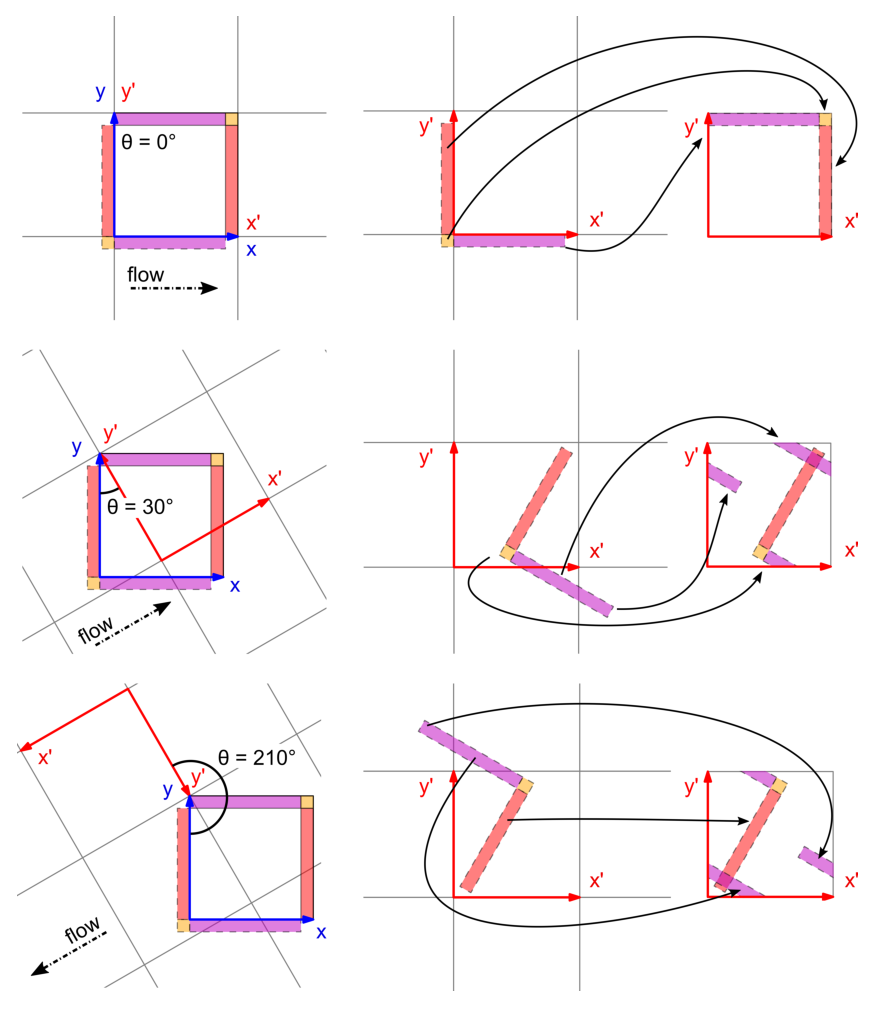
\includegraphics[width=\textwidth]{chapters/turbulent_inflow/blm/figure5.eps}
		\caption{Illustration of variable-direction concurrent precursor method for mean flow angles $\theta = 0^\circ$ (\emph{top}), $30^\circ$ (\emph{middle}), and $270^\circ$ (\emph{bottom}) with respect to the main domain x-axis. \emph{Left column: }Identification of inflow slabs (dashed colored rectangles) in precursor domains ($x'y'$) and fringe slabs (full colored rectangles) in main domain ($xy$: blue). \emph{Middle and right column: } Remapping procedure of domain-crossing inflow slabs to single precursor domain using periodic boundary conditions.}
		\label{fig:ConcurrentPrecursorRemapping}
	\end{figure}
	
	Figure~\ref{fig:ConcurrentPrecursorRemapping} illustrates cases with a set of desired inflow angles inclined at $\theta = 0^\circ$, $30 ^{\circ}$, and $210^\circ$ with respect to the main domain of interest.
	Because the precursor domain is doubly periodic, it can be continuously extended into an infinite amount of horizontally adjacent domain copies. Further, we use the convention that the mean flow in the precursor is oriented in the positive $x'$ direction. The precursor domain is hypothetically attached to the main domain at an arbitrary reference hinge point, in the illustration the top left corners of both domains (from a top view perspective), with the freedom of rotating the precursor domain around it. Inflow conditions are provided to the fringe regions of the main simulation, indicated in the left column of Figure~\ref{fig:ConcurrentPrecursorRemapping} as (``\emph{fringe slabs}''). To that end, flow field data are extracted from the (``\emph{inflow slabs}'') in the precursor simulation, also marked in the figure. From the top row of Figure~\ref{fig:ConcurrentPrecursorRemapping}, it can be seen that in the case of angle $\theta = 0 ^{\circ}$ these regions are located in the same place in both the main and precursor domain, hence the variable inflow direction concurrent precursor method becomes equivalent to the standard constant inflow angle method elaborated above in Section~\ref{sec:inflow_CP}. In the general case, the discrete locations from which inflow conditions are to be extracted do not coincide with grid points of the precursor domain. Therefore a simple second order bilinear interpolation scheme is applied. By extracting data from the dynamically moving inflow slabs, after multiplication with the classical rotation matrix
	\begin{equation}\label{eq:rotationmatrix}
	R_{\theta} = \begin{bmatrix}
	\cos \theta & - \sin \theta & 0 \\
	\sin \theta & \cos \theta   & 0 \\
	0             &  0                & 1 \\
	\end{bmatrix},
	\end{equation}
	inflow conditions can be derived for any given inflow angle $\theta$.
	
	The double periodicity of the precursor domain allows us to extract continuous inflow data from inflow slabs, even if they cross any of the horizontal domain boundaries. This is done by partitioning the inflow slab every time a domain boundary is crossed and afterwards reassembling all the regions in the correct order. This results in the complex arrangements of inflow slabs shown in the middle and right columns of Figure~\ref{fig:ConcurrentPrecursorRemapping}.
	Finally, when mapping the inflow slabs to the fringe slabs, a discontinuity in the reference velocity for the fringe regions is introduced in the corner of the main domain, as values to the north and east of the corner are respectively copied from the south-east and north-west in the inflow slabs. However, with  the use of smooth fringe forcing functions (Equation~\ref{eq:lambda}) applied to the \emph{fringe corner} region, this does not cause any issues in the simulations. Finally, note that the wide range of inflow angles shown in Figure~\ref{fig:ConcurrentPrecursorRemapping} illustrates that the proposed method does not have any restrictions on maximum/minimum angles, i.e. it can be used for any possible wind direction.
	
	\begin{figure}[ht!]
		\centering
		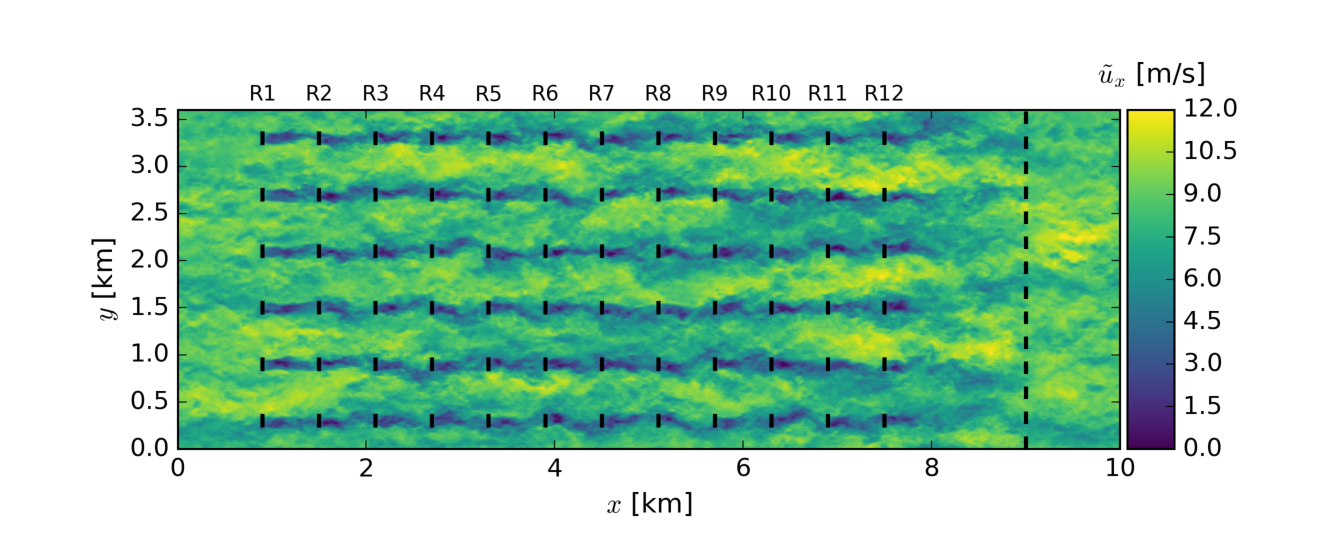
\includegraphics[width = 0.75\textwidth]{chapters/turbulent_inflow/blm/figure6.eps}
		\caption{Graphical illustration of variable inflow-direction precursor method showing contours of horizontal velocity in a neutral boundary layer. \emph{Background}: tiled precursor domains (boundaries in black), rotated to desired inflow angle. \emph{Foreground}: main domain (inside white frame). \emph{Colored patches}: fringe slabs (full lines) and inflow slabs (dashed lines). Corresponding slabs are indicated by matching face colors.}
		\label{fig:ConcurrentPrecursorField}
	\end{figure}
%%%%%%%%%%%%%%%%%%%%%%%%%%%%%%%%%%%%%%%%%%%%%%%%%%%%%%%%%%%%%%%%%%%%%%%%%%%%%%%%%%%%%%%%%%%%%%	
	\begin{figure}[h!]
		\centering
		\includegraphics[width = 0.8\textwidth]{chapters/turbulent_inflow/blm/figure7.eps}
		\caption{Dynamic action of the variable inflow-direction precursor method with a time-varying wind direction $\theta$, as seen from 2 different reference frames. \emph{Left:} Stationary main domain (white with black dashed fringe regions), rotated background precursor domains. \emph{Right:} Main domain, rotating around hinge point, on stationary background periodic precursor domains. Snapshots are separated in time by roughly 1 precursor flow-through time, as indicated by the black arrows pointing to a high speed flow region on the right panel in every snapshot.}
		\label{fig:ConcurrentPrecursorRotating}
	\end{figure}
%%%%%%%%%%%%%%%%%%%%%%%%%%%%%%%%%%%%%%%%%%%%%%%%%%%%%%%%%%%%%%%%%%%%%%%%%%%%%%%%%%%%%%%%%%%%%%
	
	\clearpage
	Figure~\ref{fig:ConcurrentPrecursorField} demonstrates the application of the method in a simulation for a flow angle of $\theta = 30^\circ$. It is observed that the fringe regions perform very well in forcing the flow field to the data extracted from the inflow slabs of the precursor simulation. Also, note the smooth transition between the precursor domain copies in the back, and the main domain.
	Figure~\ref{fig:ConcurrentPrecursorRotating} further illustrates the dynamics of the method for a changing wind direction, both seen from the precursor reference frame, and from the main reference frame.

%%%%%%%%%%%%%%%%%%%%%%%%%%%%%%%%%%%%%%%%%%%%%%%%%%%%%%%%%%%%%%%%%%%%%%%%%%%%%%%%%%%%%%%%%%%%%%	
	\begin{figure}[tb!]
					\centering
		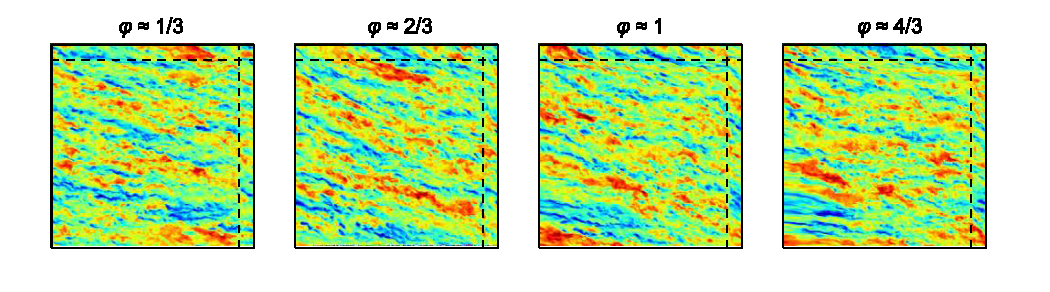
\includegraphics[width=0.9\textwidth]{chapters/turbulent_inflow/blm/figure8.eps}
		\caption{Plan view of horizontal velocity contours for different values of $\varphi$ at a height $z/H = 0.1$. The imposed flow angle has been rotated to 30$^\circ$ with a constant rate of rotation $\Omega$, varying between cases. The start of the fringe regions is indicated by the dashed black lines.}
		\label{fig:rotationrate}
	\end{figure}
	
%%%%%%%%%%%%%%%%%%%%%%%%%%%%%%%%%%%%%%%%%%%%%%%%%%%%%%%%%%%%%%%%%%%%%%%%%%%%%%%%%%%%%%%%%%%%%%
	
	The proposed approach is limited by the fact that the rotation of the main domain leads to time-varying locations of the inflow slabs in the precursor domain. This effect causes artificial compression or elongation of turbulent structures in the inflow conditions. The severity of this effect can be estimated based on the height-dependent ratio $\varphi(z) = \Omega L_h/ U_h(z) $, which should be sufficiently low. In this formula, $\Omega$ is the instantaneous imposed rate of rotation of the inflow direction, $L_h = (L_x^2 + L_y^2)^{1/2}$ is the horizontal diagonal length of the main domain and $U_h(z) = (u_x(z)^2 + u_y(z)^2)^{1/2} \approx u_x(z)$ the mean horizontal velocity at a distance $z$ from the bottom boundary in the precursor domain.
	
	In order to estimate acceptable values of the parameter $\varphi$, we illustrate the effect of the traveling motion of the inflow slabs
	qualitatively in Figure~\ref{fig:rotationrate} for several values of $\varphi$. The domain size of these simulations is $L_x \times L_y \times H
	= 2\pi \times 2\pi \times 1$ km$^3$. It can be observed from the figure that, for $\varphi \geq 1$, the turbulent structures become elongated
	and distorted (especially visible in the left-bottom corner of the domain). The severity of this distortion increases with increasing $\varphi$. It can therefore be concluded that this method is only applicable provided that the rate of change of imposed flow direction is not excessively fast compared to the time scales of the turbulence present in the flow. A conservative upper bound for sustained rotations can therefore be estimated to be $\varphi = 2/3$.
	
	As a final note, we remark that the current methodology may not be the only feasible approach to generalize precursor methods for varying wind
	directions. In fact, in a first attempt, we focused on varying the driving pressure gradient in the precursor domain. Such an approach has
	been employed for steady wind-direction simulations of an Ekman spiral by \cite{goit2013effect}, \cite{sescu2014control}, and \cite{allaerts2015large} to reorient the flow to a desired direction at a given height in the spiral. Unfortunately, in unsteady situations, this leads to a large phase-lag between the pressure gradient and the mean flow direction (that could be as long as hours), so that we did not further explore this route.

	\subsection{Horns Rev wind farm demonstration case}\label{subsec:timevaryingHR}
		
		In this section the proposed  concurrent precursor method is used in the context of a sample application where variability in inflow direction is particularly important. As mentioned before such conditions are necessary in modeling wind farms placed in the ABL subjected to possible mesoscale variability. We illustrate the method for modeling a real wind farm, namely the Horns Rev offshore wind farm located about 15 km off the Danish western coast. This wind farm has been subject of many research studies, both numerical and experimental  \cite[see, e.g.,][]{barthelmie2007modelling, pena2012atmospheric, hansen2012impact, porte2013numerical}.
		
		\subsubsection{Case Description and Numerical Setup}
		
		The farm consists of 80 Vestas V80-2MW turbines with a hub height of $z_h$ = 70 meters and a rotor diameter $D = 80$ m. The simulation
		domain is illustrated in Figure~\ref{fig:hornsrevlayout}.  The turbines are laid out as an oblique $8 \times 10$ rectangle, sheared with
		approximately 7$^\circ$ with respect to the north-south line. We refer to a group of turbines located on the same east-west line as a
		column. Likewise, a group of turbines on a north-south line (with a 7$^\circ$ angle) is denoted as a row. Turbines are spaced apart
		approximately 7$D$ in both the streamwise (east-west) and spanwise (north-south) direction. The turbines are represented in the
		simulation using an actuator disk model (see Section~\ref{sec:meth_adm}) with a constant $\widehat{C}_T' = 1.53$, corresponding to a
		thrust coefficient $C_T = 0.8$ (see, e.g. \citealp{wu2015modeling,stevens2015using}). The  dimensions of the main simulation domain are $L_x = L_y = 10$ km in the horizontal directions and $L_z = 1$ km in the vertical direction. This relatively large domain
		rules out any possible upstream influence of the fringe regions on the farm \citep{lundbladh1999efficient,nordstrom1999fringe}.
		
		\begin{figure}[h]
			\centering
			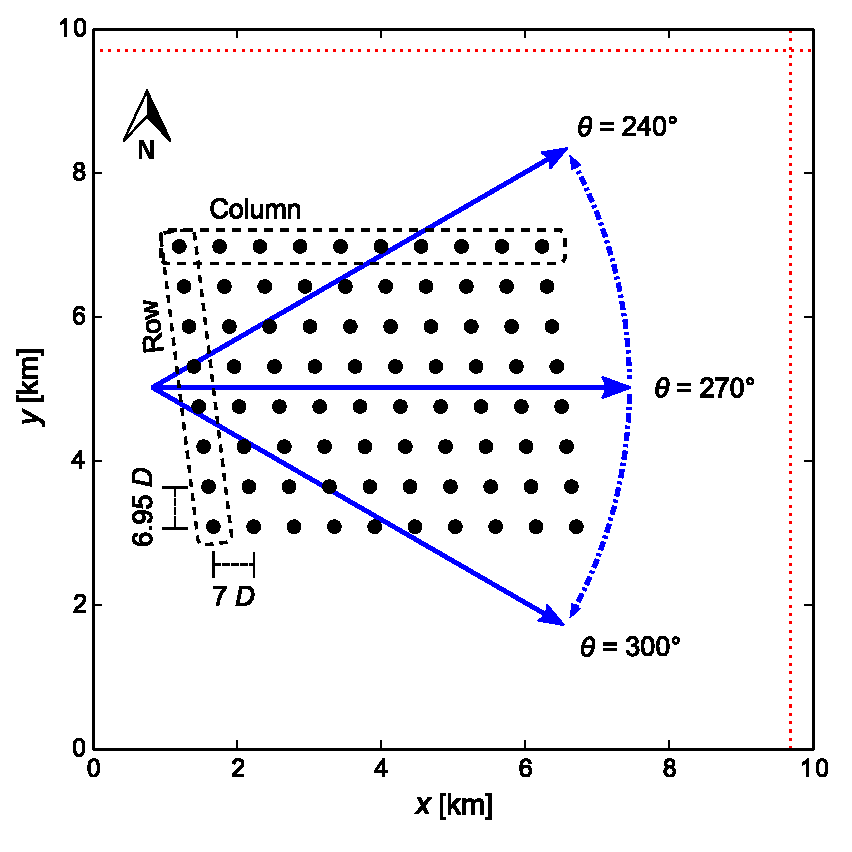
\includegraphics[width=0.75\textwidth]{chapters/turbulent_inflow/blm/figure9.eps}
			\caption{Simulation domain for Horns Rev wind farm. The location of the turbines is indicated with black circles. The dashed-red lines indicate the start of the fringe regions.}
			\label{fig:hornsrevlayout}
		\end{figure}

		A uniform grid of $768 \times 768 \times 192$ grid points is used in the main domain, and the same grid size is used for the precursor domain. This leads to a resolution of $\Delta_x = \Delta_y$ = 13 m in the horizontal directions and $\Delta_z$ = 5.21 m in the vertical direction. The timestep is restricted by a CFL limit, and fluctuates around 0.6 seconds. Inflow conditions are generated by a parallel auxiliary precursor simulation, as discussed in previous sections. Details of the case setup are further summarized in Table~\ref{tab:simulationparameters}.
		
		In the simulations, the turbines are yawed such as to track the incident wind direction. The yaw controller is based on the heuristic baseline controller developed by \cite{kooijman2003dowec}, and later successfully applied by \cite{storey2014modelling} in wind-farm LES. Whenever 90 second or 5 second running average yaw errors exceed 5$^\circ$ or 30$^\circ$ respectively, the turbine starts yawing at a constant speed of $0.1^\circ/\text{sec}$ to compensate the offset, until the 5 second yaw error drops below 0.5$^\circ$.
		
		Simulation results are non-dimensionalized with the domain height $H$ = 1000 m, and a friction velocity of $u_* = 0.357$ m s$^{-1}$. This leads to a wind speed of approximately 8 m s$^{-1}$ at hub height ($z = 70$ m), upstream of the farm. In this study, we select a roughness length $z_0 = 0.01$ m. Even though this value is significantly higher than the roughness length observed in typical offshore conditions, the resulting observed turbulence intensity TI at hub height is approximately 7.5\%. This is close to prior numerical studies \citep{porte2013numerical, wu2015modeling} and experimental observations \citep{barthelmie2009modelling, barthelmie2010quantifying} for the Horns Rev wind farm, where TI was found to be less than 8\% for neutral atmospheric conditions. TI is defined here as $(\langle \overline{ u_i' u_i'} \rangle /3)^{1/2} / \langle \overline{u}_{hub} \rangle$, where brackets and overline denote horizontal and time-averaging operators respectively.
		
		First, a statistically steady turbulent boundary layer is created by spinning up the precursor simulation from random perturbations for a time period corresponding to slightly over 20 physical hours. Afterwards, the generated field is used in both the precursor and main simulation domain. The turbines are then inserted in the main domain, and the flow is further advanced in time for roughly 1 hour, so that the wind farm in the main domain also attains statistical equilibrium. This point in time is denoted as  $t = 0$ in all figures and discussion.
		
		We consider a set of simulations in which the mean wind direction is varied sinusoidally in time as $\theta(t) = 270^\circ - 30^\circ
		\sin(2\pi t/T_\theta)$, where the period of the sine wave $T_\theta$ equals 1 hour (case \emph{V}1), 2 hours (case \emph{V}2), and 4 hours (case \emph{V}4). Moreover, we define a set of reference cases with a steady mean wind direction in the sector around the 270$^\circ$ (westerly) wind direction. This set consists of 15 separate LESs for mean wind directions as indicated in Table~\ref{tab:simulationparameters}, and are referred to as \emph{ST} in the remainder of this text. Cases \emph{V}1, \emph{V}2, \emph{V}4 and \emph{ST}270 are simulated for a time horizon of 4 hours, whereas the other steady cases (\emph{ST}) are performed for a period of 2 hours. For the variable cases \emph{V}4, \emph{V}2, and \emph{V}1, the imposed rotation rates lead to average ratios $\varphi$ of approximately 0.25, 0.5, and 1, respectively. Note that, for case \emph{V}1, $\varphi$ is higher than our conservative upper bound estimate of 2/3 (see further discussion below).
		
		\begin{table}
			\centering
			\begin{tabularx}{\textwidth}{Xl}
				\hline
				\rule{0pt}{2.8ex}Domain size                             & $L_x \times L_y \times H = 10 \times 10 \times 1$ km$^3$ \\
				Turbine dimensions                      & $D = 80$m, $z_h = 70$m \\
				Turbine arrangement                     & $10$ (E-W) $\times 8$ (N-S) (see Figure~\ref{fig:hornsrevlayout})\\
				Turbine spacing                         & $S_x = 7D$ (E-W), $S_y = 6.95D$ (N-S) \\
				Surface roughness                         & $z_0 = 0.01$m  \\
				Grid size in main//precursor             & $N_x \times N_y \times N_z = 768 \times 768 \times 192$ // $768 \times 768 \times 192$ \\
				Cell size                                   & $\Delta_x \times \Delta_y \times \Delta_z \approx 13 \times 13 \times 5.2$ m$^3$ \\
				Timestep                                & $\Delta t \approx 0.6$ s\\
				%    Wind direction (steady)            & \red{$\theta = 270^\circ$, $270^\circ \pm 1^\circ$,$ \pm 3^\circ$,$\pm 5^\circ$,$\pm 10^\circ$,$\pm 15^\circ$,$\pm 20^\circ$,$\pm 30^\circ$} \\
				Wind direction: steady \emph{ST}            & $\theta = 270^\circ$, $271^\circ$, $273^\circ$, $275^\circ$, $280^\circ$, $285^\circ$, $290^\circ$, $300^\circ$,  \\
				& \qquad \quad $269^\circ$, $267^\circ$, $265^\circ$, $260^\circ$, $255^\circ$, $250^\circ$, $240^\circ$\\
				Wind direction: time-varying \emph{V}      & $\theta = 270^\circ - 30^\circ\sin(2\pi t/T_\theta) $\\
				& \qquad \quad $T_\theta = 1$h (\emph{V}1), $2$h (\emph{V}2), $4$h (\emph{V}4) \\
				\hline
			\end{tabularx}
			\caption{Summary of simulation setup parameters}
			\label{tab:simulationparameters}
		\end{table}
		
		
		
		
		\subsubsection{Results}
		First a set of steady cases (\emph{ST}) in a 270$^\circ$ (westerly) wind direction sector is discussed, and compared to experimental
		and simulation data from literature. Results of variable wind-direction cases  (\emph{V}) are presented afterwards.
		Figure~\ref{fig:hornsrevsteady} shows the extracted power for a 270$^\circ$ mean wind direction, obtained from the case \emph{ST}270,
		averaged over each turbine row and normalized by the first row. This particular wind direction is well documented in literature, with
		experimental power measurements from the SCADA data of the Horns Rev wind farm \citep{barthelmie2009modelling,barthelmie2010quantifying}. Previous LES results are also shown  \cite{ivanell2009numerical,porte2013numerical}. It is appreciated in Figure~\ref{fig:hornsrevsteady} that our simulation results show relatively good agreement with the experimental data, as well as with the LES data from \cite{porte2013numerical}. The main discrepancies with the latter occur in the entrance region of the wind farm, i.e. in the second and third rows. This is related to the use of a different subgrid-scale model, and a different ADM in our code: Port\'e-Agel \emph{et al.} use a scale-dependent dynamic Smagorinsky model which is known to be less dissipative than our standard Smagorinsky model. They further also use a more advanced rotating actuator disk implementation. Further downstream, our results closely match Port\'e-Agel \emph{et al.}'s results, as well as the Horns Rev measurement data. For sake of reference, the results reported by \cite{ivanell2009numerical} are also included in Figure~\ref{fig:hornsrevsteady}. These results were obtained using the Mann spectral model for the generation of inflow turbulence, and it is appreciated that this leads to a significant underprediction of power extraction. Later, this was attributed to a decreased triggering of wake meandering by Mann turbulence compared to precursor generated turbulence \citep{churchfield2012large}. 
		
		\begin{figure}[ht]
			\centering
			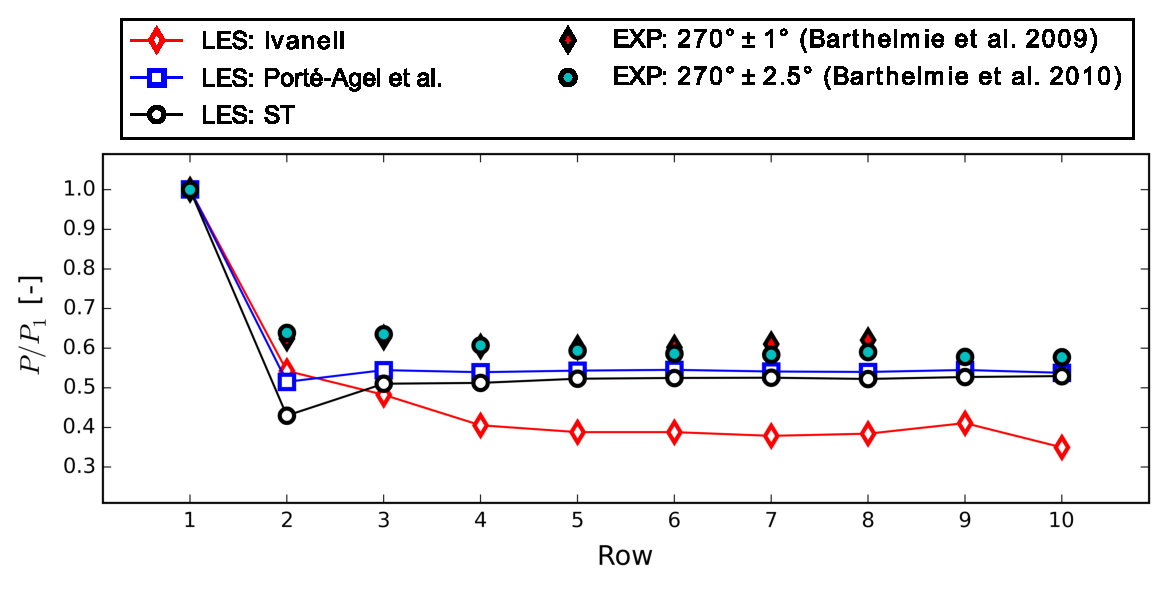
\includegraphics[width=0.99\textwidth]{chapters/turbulent_inflow/blm/figure10.eps}
			\caption{Normalized power as function of row number.
				Numerical reference data from \cite{ivanell2009numerical} and \cite{porte2013numerical}, and experimental measurements from \cite{barthelmie2009modelling, barthelmie2010quantifying} are included. }
			\label{fig:hornsrevsteady}
		\end{figure}
		
		Figure~\ref{fig:topviewfarms} shows top views of the flow field for the different variable wind-direction cases (\emph{V}1, \emph{V}2, \emph{V}4) at different time instances to illustrate the flow behavior for different wind directions. As can be expected, the distance over which the wakes are able to recover before they hit the next turbines changes significantly with wind direction, and thus time into the simulation. Further focusing on case \emph{V}1, for which $\varphi\approx 1$ is slightly too high compared to our estimated upper limit  $\varphi \leq 2/3$  in Section~\ref{subsec:timevaryingCP}, we do not observe the type of severe distortions of turbulent structures that we found earlier in Figure~\ref{fig:rotationrate} for too high rotation rates. However, when looking at the full range of snapshots for this case (not shown here), distortions are sometimes visible for short times near the edges of the computational domain, but they do not seem to affect the main features of the flow in the wind farm itself. This confirms however the estimate $\varphi \leq 2/3$ discussed in Section~\ref{subsec:timevaryingCP}.
		
		Figure~\ref{fig:timeyaw_timepower} contains a summary of simulation results for the variable wind-direction cases (\emph{V}). From the
		top row, it can be appreciated that the mean yaw angle in the wind farm follows the imposed  wind direction closely for all cases,
		although some overshoots are observed for case \emph{V}1. The middle row shows aggregate power output as a function of time, combined
		with the case \emph{ST}270. The increased variability of aggregate farm power for the variable wind-direction cases is mainly caused
		by the strong sensitivity of power extraction to mean wind direction, as is well known from previous studies (see, e.g. \citealp{barthelmie2010quantifying, porte2013numerical}). Moreover, it is shown that the faster-varying cases \emph{V}1 and \emph{V}2 exhibit significant hysteresis effects, i.e. the waveforms of aggregate power show a strong asymmetry with leading peaks. The slowly-varying case \emph{V}4 shows a more symmetric pattern.
		
		The bottom row of Figure~\ref{fig:timeyaw_timepower} shows aggregate power as a function of mean wind direction. Time-averaged wind-farm power extractions obtained from the steady wind-direction cases (\emph{ST}) are also shown. As may be expected, time-varying simulation results increasingly correspond to steady state cases when the rate of rotation is decreased. However, the hysteresis effects of the faster rotation cases are also clearly visible. Moreover, all cases show significant undershoots in power extraction around the fully-waked $270^\circ$ conditions. This is further explained based on Figure~\ref{fig:explanation_undershoot} for case \emph{V}2. The figure compares an instantaneous flow field from a steady $270^\circ$ simulation to the $270^\circ$ solution from the unsteady case after 4 hours. It is observed that in the steady wind-direction simulation, high-speed channels in between the turbine columns are much more pronounced and penetrate much deeper into the farm. This can be explained by the changing wind direction in the variable case, which much better mixes the high-speed regions with the low speed regions between the turbines. As a result, at an earlier stage in the simulation ($\theta \neq 270^\circ$) the available inflow energy in the farm was better captured by the first rows of turbines, leaving less energy in the `high-speed' channels near the end of the farm at the later $\theta=270^\circ$ instance. The reduced power extraction for the variable cases at $270^\circ$ (observed in Figure~\ref{fig:timeyaw_timepower}) is a result of this process.
		
		\begin{figure}[ht]
			\centering
			\includegraphics[width = \textwidth]{chapters/turbulent_inflow/blm/fig11_smaller}
			\caption{Planview of instantaneous flow field at hub height for variable wind-direction cases at 3 time instances visualized using contours of horizontal velocity magnitude. \emph{Top: } \emph{V}1. \emph{Middle: } \emph{V}2. \emph{Bottom: } \emph{V}4. The units on the color bar are m s$^{-1}$.} 
			\label{fig:topviewfarms}
		\end{figure}
		
		
		\begin{figure}[ht]
			\centering
			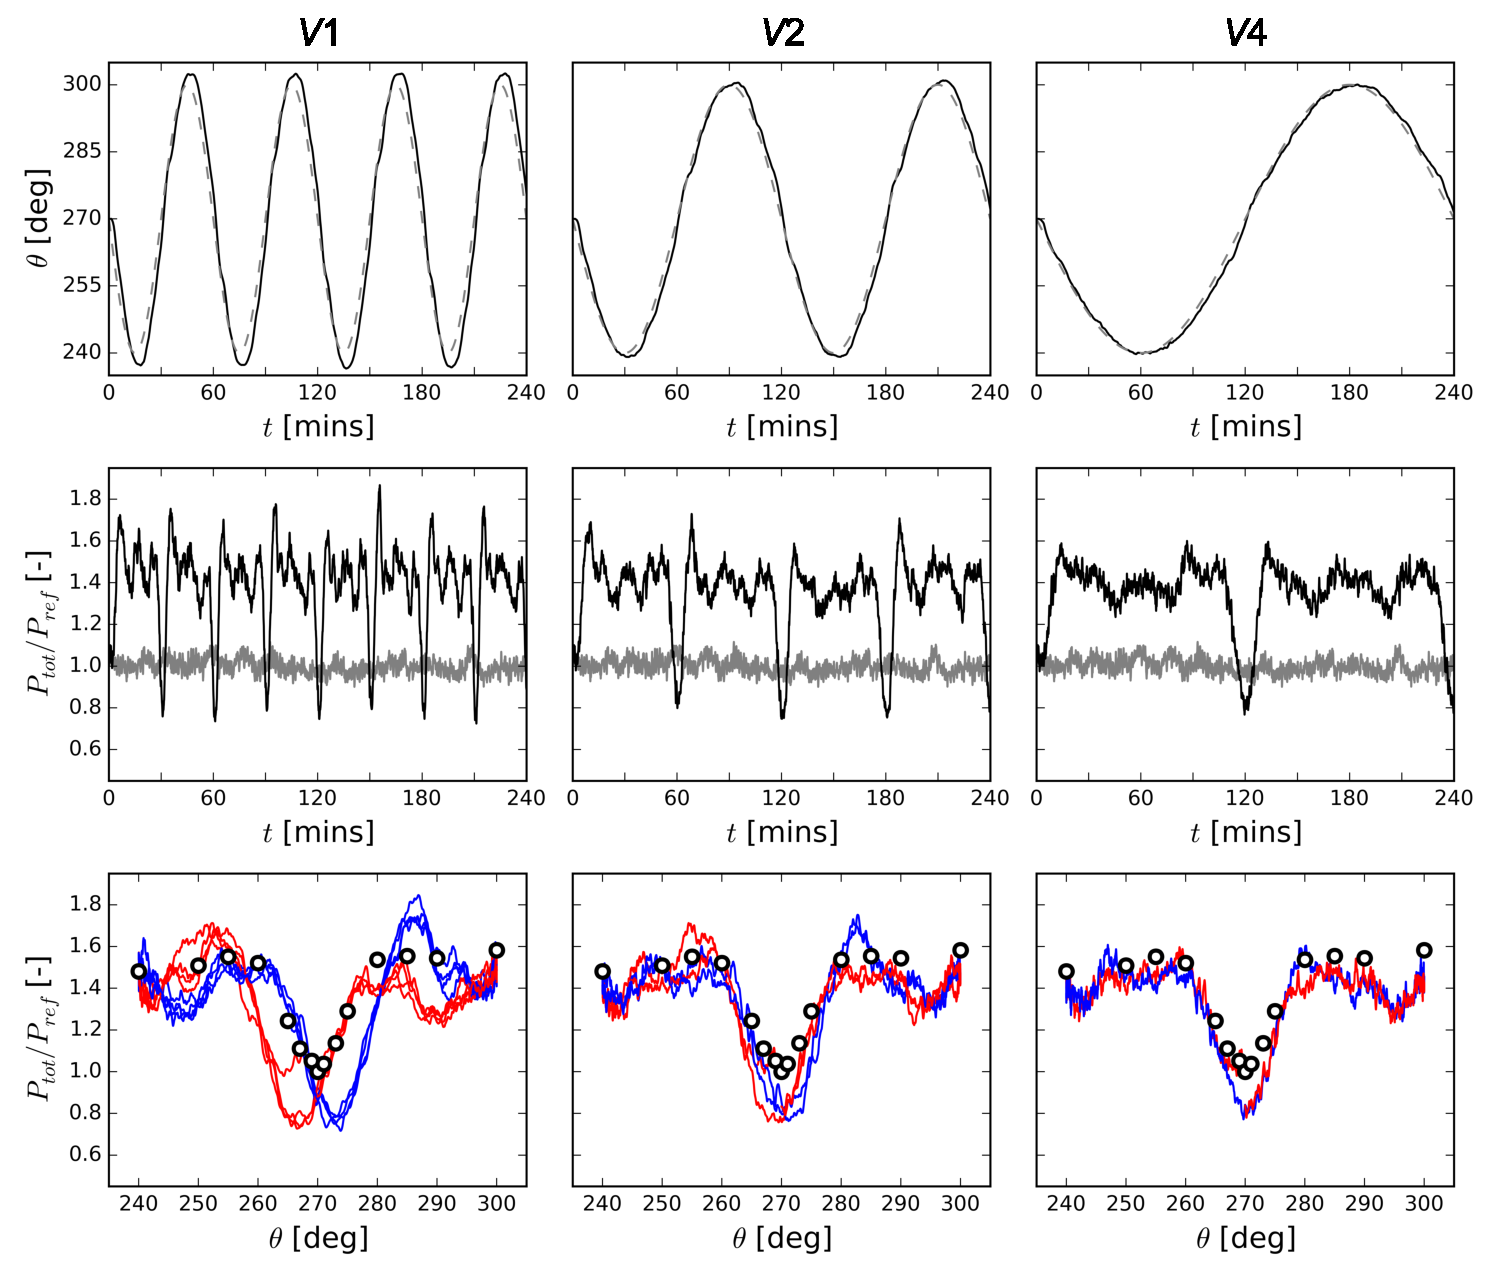
\includegraphics[width=\textwidth]{chapters/turbulent_inflow/blm/figure12.eps}
			\caption{Simulation results for case \emph{V}1 (\emph{left}), \emph{V}2 (\emph{middle}), and \emph{V}4 (\emph{right}). \emph{Top}: Imposed wind direction (dashed lines) and resulting mean turbine yaw angle (full lines). \emph{Middle}: Aggregate wind-farm power extraction, along with case \emph{ST}270, normalized by time-averaged \emph{ST}270 power. \emph{Bottom:} Aggregate wind-farm power extraction as a function of mean flow angle for the time-varying wind direction cases (lines), as well as a set of steady state cases at several mean flow angles (circles). Red and blue lines indicate time periods during which $d\theta/dt > 0 $, and $d\theta/dt < 0$ respectively. Power is normalized by time-averaged \emph{ST}$270$ power.}
			\label{fig:timeyaw_timepower}
		\end{figure}
		
		Figure~\ref{fig:spectra_power} shows time spectra $\phi$ of the aggregate power extracted by the wind turbines from the boundary-layer flow for case \emph{ST}270, \emph{V}1, \emph{V}2, and \emph{V}4. It is observed for frequencies higher than 0.02 Hz that all cases show identical spectral behavior Results show a Kolmogorov-type $-5/3$ scaling range, which transitions to a $-1$ range at lower frequencies. Moreover, the spectrum  of case \emph{ST}270 exhibits a spectral peak in the frequency range around $10^{-2}$ Hz, which is directly related to the time for the flow to proceed from one row of turbines to the next. The existence of the peak is caused by the correlation between extracted power of turbines within the same column, which in turn is due to the advection of large scale streamwise-oriented turbulent structures. For a more detailed analysis of this phenomenon, we refer the reader to \cite{stevens2014temporal} and \cite{bossuyt2017wind}. In the variable wind-direction cases, the peak is smeared out as the turbine-to-turbine flow time no longer corresponds to a narrow frequency band. These cases also exhibit increased energy at the low frequency part of the spectrum, caused by the single-frequency variation in wind direction. This is also shown in the time series of aggregate farm power in Figure~\ref{fig:timeyaw_timepower}.
		
		\begin{figure}[ht]
			\centering
			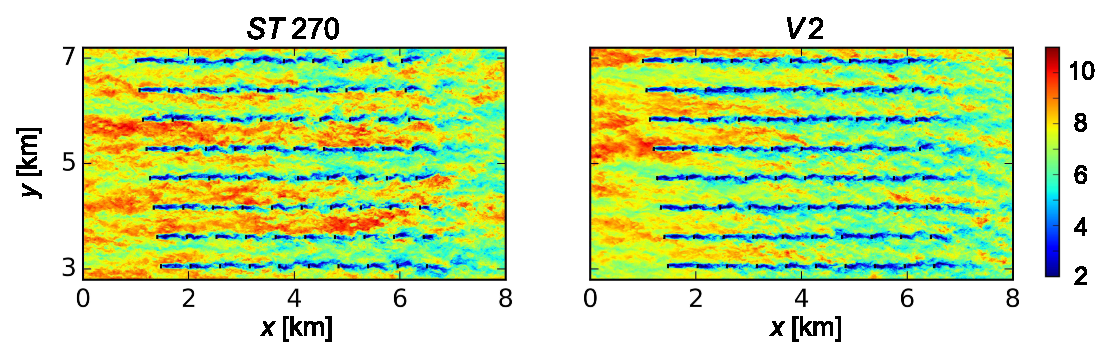
\includegraphics[width=\textwidth]{chapters/turbulent_inflow/blm/fig13_3}
			\caption{Plan views of instantaneous horizontal velocity magnitude at turbine hub height for $\theta = 270^\circ$. \emph{Left: } Steady state case \emph{ST}270. \emph{Right: } Variable wind-direction case \emph{V}2 at $t$ = 4 hours.}
			\label{fig:explanation_undershoot}
		\end{figure}
		
		\begin{figure}[ht]
			\centering
			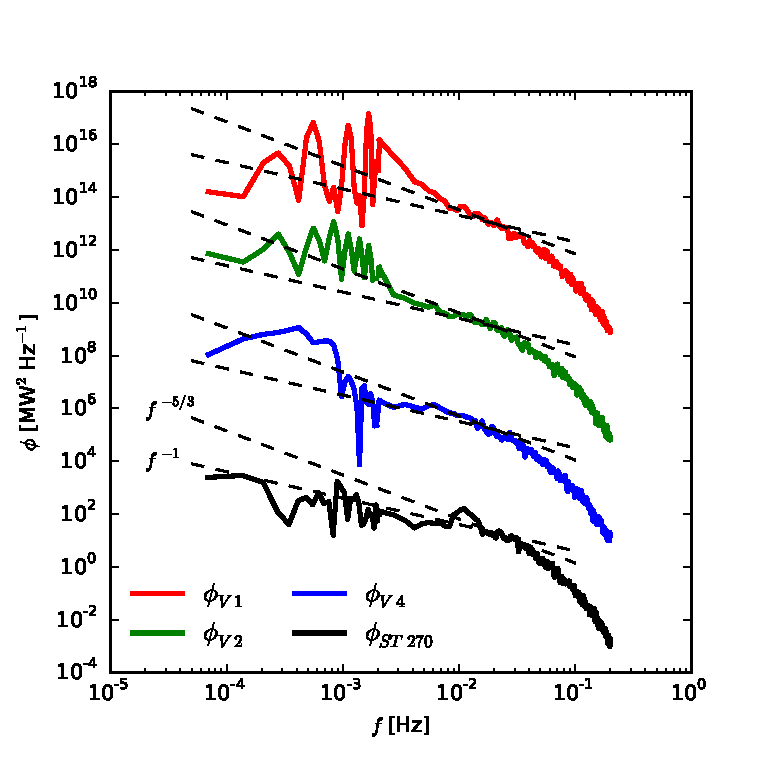
\includegraphics[width=0.75\textwidth]{chapters/turbulent_inflow/blm/figure14.eps}
			\caption{Time spectra of extracted power $\phi$ for the cases \emph{ST}270, \emph{V}1, \emph{V}2, and \emph{V}4. Cases shifted vertically for clarity of presentation. Spectra for frequencies $f > 2 \times 10^{-3}$ Hz are calculated using Welch's periodogram method for better statistical convergence. }
			\label{fig:spectra_power}
		\end{figure}
		
		
		In summary, the current section provides a demonstration case for the variable inflow-direction concurrent precursor method presented in this chapter. A set of steady state reference cases at different wind directions is defined with the aim of illustrating hysteresis effects in power extraction for the variable wind-direction cases. As the rate of rotation is decreased, the latter show increased correspondence with the reference cases. However, even case \emph{V}4, which exhibits the slowest variations, displays an undershoot at $\theta = 270^\circ$, compared to the steady state case \emph{ST}270. Even though time series of extracted farm power appear very different qualitatively, spectral behavior at higher frequencies is found to be identical.
		
		
	\subsection{Interim summary}
	The current chapter addresses the long-standing issue of the generation of inflow conditions for turbulence-resolving flow simulations.
	The importance of high quality inflow turbulence has been reaffirmed based on a literature review and presentation of a qualitative comparison
	between precursor methods and a sample of synthetic inflow methods.  While precursor techniques are the only methods capable of producing
	large-scale coherent structures and display the best quality overall, classical implementations lack the flexibility to apply them to flow
	cases involving variable mean inflow directions. To circumvent this limitation, a variable-direction precursor method has been developed and
	implemented in the SP-Wind LES solver. The approach can provide fully-developed turbulent inflow conditions to turbulence-resolving
	simulations  for variable wind directions at a computational cost which does not exceed the cost of classical precursor techniques.  The
	method is relatively general as it can be applied to LES or DNS whenever variable inflow conditions are prescribed, provided the rate of change of imposed flow direction is not excessively fast compared to the time scales of the turbulence in the main domain of interest.
	
	The proposed method was applied to a set of 3 LESs of the Horns Rev wind farm, subject to an imposed hypothetical sinusoidal variation in wind direction with an amplitude of $\pm 30^\circ$ and time periods of 1, 2, and 4 hours respectively. A comparison with steady state simulations illustrated that the faster-varying cases exhibit significant hysteresis effects in power extraction. Moreover, all variable wind-direction simulation cases show an undershoot of power production at westerly $270^\circ$ winds, compared to steady state conditions. Finally, even though time series of extracted power appear very different qualitatively, spectral behavior at higher frequencies was found to be identical.

	\clearpage
	
\section{Spanwise locking and shifted periodic boundary conditions}\label{sec:inflow_shifted}
It was mentioned before that periodic boundary conditions provide an efficient means of achieving fully-developed turbulent inflow conditions by recycling turbulent fluctuations from the domain outlet back to the inlet. In this way, spinning up fully-developed turbulence from random initial perturbations can occur over time instead of having to resolve spatial transition using an elongated simulation domain. This explains why the approach is mostly the method of choice for simulation of fully developed boundary layer flows, such as DNS of turbulent channel flows \citep{kim1987turbulence}, pipe flows \citep{monty2007large,wu2008direct} Couette flows \citep{takahiro2006dns} etc., and similar studies based on LES. Moreover, as discussed in Section~\ref{sec:inflow_intro}--\ref{sec:inflow_var}, periodic boundary conditions are also often applied in precursor simulations for the generation of fully developed inflow turbulence for streamwise developing wall-bounded flows \citep{tabor2010inlet, stevens2014concurrent}.

When using periodic boundary conditions to generate fully developed turbulence, any nonphysical influence originating from the perfect correlations
over the periodic domain length should be avoided. To this end, the size of the computational domain should be chosen to be several times larger than
the largest scales in the flow. In boundary layers, experimental and numerical studies have shown the existence of very large streamwise-elongated
coherent structures, with length scales of the order of tens of boundary layer thicknesses $\delta$ (see, e.g., \citealp{delalamo2003spectra,
tomkins2003spanwise, hutchins2007evidence}). These structures are ubiquitous in neutral wall-bounded flows, ranging from lower Reynolds number
laboratory-scale flows to the high Reynolds number ABL \citep{balakumar2007large,hutchins2012towards}. In the literature, these streaky structures are
commonly referred to as superstructures \citep{hutchins2007evidence} or Very-Large-Scale Motions (VLSM) \citep{kim1999very, fang2015large}. As a
consequence of these very long structures, domain lengths $L_x$ in streamwise periodic wall-bounded turbulent flow simulations may need to be on the
order of $L_x=32\pi\delta$ to  $60\pi\delta$, in order to fully capture them \citep{lozanoduran2014effect,fang2015large}.

At these domain lengths, simulations become very expensive, and lack of computational resources has often led to the use of domain sizes that are much
smaller, e.g., $L_x=2\pi\delta$ is a choice often encountered in the literature. However at too short domain lengths, superstructures lack the
streamwise space to significantly meander or break up before they are recycled back to the inlet. Thus, they become virtually infinitely long, and
remain locked in time at the same spanwise position by the persistent recycling. Simulation results of spanwise-homogeneous flows in too short domains
are therefore biased to have sustained streamwise-oriented bands of high and low speed velocity, even after very long time averaging (see, e.g.,
\citealp{lu2010modulated, verhulst2014large, alqadi2015large}). As, e.g., discussed by \cite{lozanoduran2014effect} these quasi-infinite structures in
too short simulation domains do ``capture most of the effects of the actual structures, or at least of their interactions with smaller scales of size
$\mathcal{O}(\delta)$.'' As a result, horizontally and time averaged profiles are not affected (as also shown below). However, this
persistent spanwise inhomogeneity is very important in cases where the fully developed turbulence in a precursor simulation is used as an inlet
boundary condition to a simulation which is not homogeneous in the spanwise direction. This problem is illustrated Figure
\ref{fig:inflow_illustrate_lock}, where a precursor simulation with a streamwise extent $L_x=2\pi\delta$ was used to generate turbulent inflow for a
wind-farm simulation. The figure depicts time-averaged streamwise velocity and mean power extraction by each of the 12 turbine columns, normalized by
mean farm power. Statistics were gathered over a time period of slightly over 8 physical hours. It can be observed from the figure that, although the
wind farm is spanwise homogeneous, different turbine columns are subjected to different inflow conditions, resulting in significant spurious variations in power extraction. 
The locking phenomenon has also been investigated by \cite{fishpool2009persistent} for channel flows at $Re_\tau$ = 180 and 410, with streamwise
domain lengths $L_x = 4\pi\delta$ and $2\pi\delta$ respectively. It was found that, in both flow cases, the locking effect led to significant spanwise
variations in time-averaged velocity. In the current section, we propose a \emph{shifted periodic boundary condition} which, in contrast to classical
periodic boundary conditions, adds a spanwise offset (i.e. shift) to the outflow plane before reintroduction at the inlet, to remedy this problem. 

\begin{figure}
	\centering 
	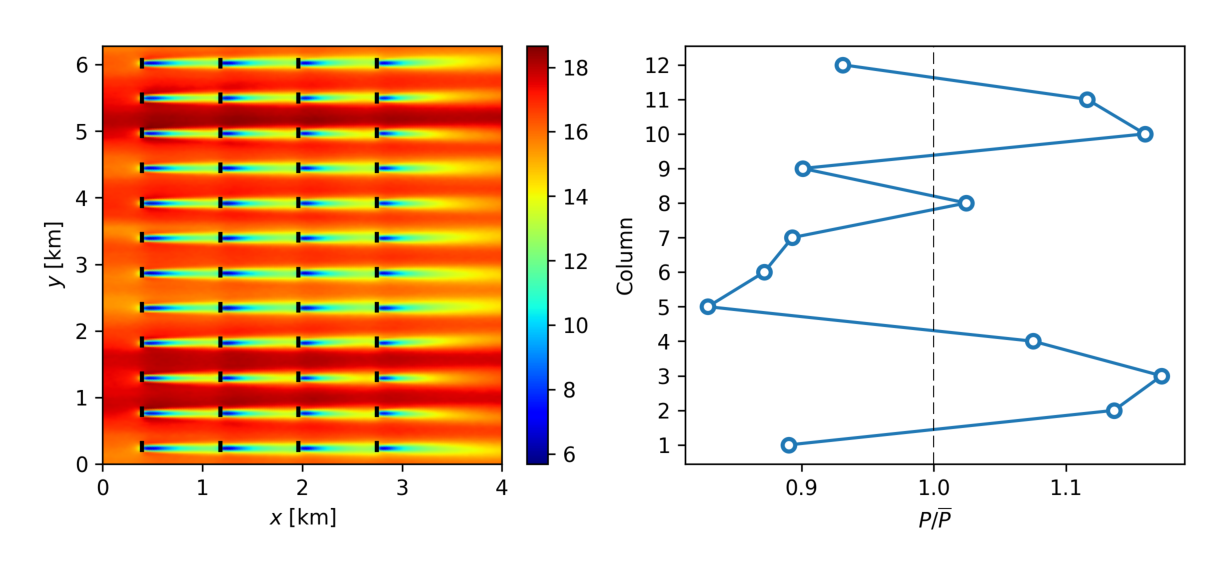
\includegraphics[width=\textwidth]{chapters/turbulent_inflow/illustrate_lock}
	\caption{Illustration of spanwise locking effect in precursor simulations for wind-farm LES. \emph{Left: } Time-averaged streamwise velocity at hub height, with inflow generated from a separate precursor simulation using $L_x=2\pi\delta$. \emph{Right: } Time-averaged mean power extraction per column, normalized by mean wind-farm power extraction. \label{fig:inflow_illustrate_lock}}
\end{figure}

Firstly, the method and its implementation in a pseudo-spectral discretization is discussed in Section~\ref{sec:inflow_shifted_shifted}. Next, the efficacy of the method is illustrated based on an application to canonical wall-bounded turbulent flow simulations in Section~\ref{sec:inflow_shifted_application}. Thereafter, the boundary conditions are applied in a precursor method, providing inflow for a spatially developing wind-farm boundary layer in Section~\ref{sec:inflow_shifted_demo}.

	\subsection{Shifted periodic boundary conditions}\label{sec:inflow_shifted_shifted}
	Here, we elaborate on a \emph{shifted periodic boundary condition} approach that prevents the spanwise locking of large-scale structures in simulation domains that are too short. The methodology is illustrated in Figure~\ref{fig:concept}. Instead of straightforwardly reintroducing the velocity from the outlet plane back at the inlet, this plane is first shifted uniformly in the spanwise direction by a predefined and constant distance $d_s$. 
	
	The shifting distance $d_s$ is the only user-defined parameter in the method. The main constraint for choosing $d_s$ is to avoid
	reintroduction of turbulent structures by the shifting operation at exactly the same spanwise location after only a limited number of
	flowthroughs. Since spanwise boundary conditions remain periodic, such a situation would occur after $N$ flowthroughs, where $N d_s = M L_y$
	with $N$ and $M$ integers. Mathematically, this means that the ratio $L_y/d_s$, when expressed as a simple fraction of integers in its lowest
	terms, should have a large numerator. Equivalently, $d_s$ and $L_y$ should have a large least common multiple to assure a large $N$. This is
	illustrated graphically in Figure~\ref{fig:topview_shift} for $d_s = \delta/2$ and $d_s = L_y/2$. The figure shows adjacent copies of velocity field planviews, shifted in the spanwise direction with the respective $d_s$ at the streamwise domain boundaries. The arrows illustrate where turbulent structures will be reintroduced after flowing through the domain. It can be observed from the figure that choosing $d_s = L_y/2$ results in structures arriving at the exact same spanwise location after only 2 flowthroughs.
	
	In practice, we propose to choose $d_s$ such that it flattens out the spanwise variations as quickly as possible. 
	Therefore, we choose a value of $d_s = 0.5\delta$ since this is roughly equal to the spanwise lengthscale of the largest turbulent structures in the wall-bounded flows studied here \citep{tomkins2003spanwise, hutchins2007evidence,fang2015large}. 
	In this way, the large-scale structures gradually sweep the spanwise extent of the domain. 
	Note that this lengthscale is dependent on factors such as Reynolds number and distance to the wall. 
	Therefore, we verified that other values also yield satisfactory results with significant reductions in spanwise inhomogeneities (e.g. $d_s = \delta/4$, $\delta$, $3\delta/2$), provided that $d_s$ and $L_y$ have no ``small'' least common multiple.
	
	The spanwise domain boundaries are still treated with standard periodic boundary conditions. This allows us to reconstruct a continuous inflow plane at the streamwise inflow boundary since, after shifting, the portion of the outflow plane which falls out of range can now be remapped to the other side, as shown by the dashed arrows and the indicated flow structure in Figure~\ref{fig:concept}b. The methodology, although conceptually simple, leads to significant improvements in the spanwise homogeneity of time-averaged flow fields, as is shown below.
	
	For standard numerical discretizations, e.g. by the finite-difference of finite-volume approach, the proposed shifted periodic boundary
	conditions can be straightforwardly imposed in a similar way as traditional periodic boundary conditions, albeit with a spanwise shift.
	However, in turbulent flow simulations,  spectral methods are often the method of choice due to their high accuracy. As discussed in Section
	\ref{sec:meth_discr}, this is also the case here, as we apply a Fourier pseudo-spectral discretization in the horizontal directions. Note that
	this discretization requires true global periodicity, and is hence incompatible with a direct implementation of shifted periodic boundary
	conditions. As shown in Figure~\ref{fig:concept}c an auxiliary region is appended to the back side of the original simulation domain. At the
	end of the extended domain a fringe region is defined (see Section~\ref{sec:meth_fringe}), in which the Navier--Stokes solution is smoothly
	nudged towards a spanwise-shifted version of the flow field at the original effective domain length $x = L_{\textit{\small x,eff}}$. The
	outflow is then reintroduced at the domain inlet through the global periodic boundary conditions. The solid arrows in Figure~\ref{fig:concept}
	summarize the flow of information as discussed above. Note that, in contrast to traditional periodic boundary conditions, in the current
	implementation there is no direct feedback from the flow field at the inlet of the domain (at $x=0$) to the flow field at the ``effective'' outlet of the domain (at $x=L_{\textit{x,eff}}$). 
	
	As discussed in Section~\ref{sec:meth_discr}, similar to the velocity field, the pressure field is also decomposed into Fourier modes, hence the pressure field is also subjected to globally periodic boundary conditions. In case the currently proposed shifted boundary conditions are implemented in a standard flow solver, for which the Poisson equation requires appropriate pressure boundary conditions, the same spanwise-shifted periodic boundary conditions, as used for velocity, can be applied for pressure as well.
	
	\begin{figure}
		\centering
		\includegraphics[width=\textwidth]{chapters/turbulent_inflow/spbc/figure1}
		\caption{Visualization of shifted periodic boundary condition concept for a turbulent half-channel simulation. The flow direction is indicated by the blue dashed arrows. \emph{a)} Classic periodic boundary conditions. \emph{b)} Shifted periodic boundary conditions, $d_s$ indicates shifting distance. Original (pre-shift) spanwise domain boundary indicated by black dot-dashed line in the inlet plane. The encircled structure illustrates how planes can be ``wrapped around'' the spanwise periodic boundary conditions. \emph{c)} Implementation in a solver with Fourier pseudo-spectral discretization in the streamwise direction, requiring global periodicity. The shaded region indicates the \emph{fringe} region.}
		\label{fig:concept}
	\end{figure}
	
	\begin{figure}
		\centering
		\includegraphics[width=0.7\textwidth]{chapters/turbulent_inflow/spbc/figure2}
		\caption{Spanwise-shifted planview copies of instantaneous contours of streamwise velocity component for a fully-developed half-channel flow at $z/\delta = 0.1$ with an effective domain length $L_{x,eff} = 2\pi\delta$. Dashed black lines indicate boundaries between domain copies. Full black lines with arrows illustrate how the shifted periodic boundary conditions relocate turbulent structures in the spanwise direction. Coloring is in units of $u/u_*$. }
		\label{fig:topview_shift}
	\end{figure}
	
	
	\subsection{Application to fully-developed wall-bounded turbulent flows}\label{sec:inflow_shifted_application}
		In order to illustrate that the locking effect is a by-product of the combination of periodic boundary conditions and an insufficient streamwise length, a suite of simulations is performed using varying streamwise domain sizes. Next to that, simulations with shifted periodic boundary conditions are also performed. The considered cases are summarized in Table~\ref{tab:cases} and consist of DNS for fully-developed channel flows (C) at $Re_\tau = 395$, and LES for fully-developed rough-wall half-channel flows (HC) at very high Reynolds number. 
		
		Both inner and outer layers of wall-bounded turbulent flows can contain long-lived structures affected by the locking effect as long as they are streamwise-elongated and roughly as large as the computational domain. \cite{fishpool2009persistent} did an analysis of the timescales towards homogeneity at different heights for a channel flow at $Re_\tau = 410$, similar to the channel (C) DNS included below. Also, \cite{fang2015large} studied the behavior of VLSM in the ABL at different distances from the wall using a simulation setup closely resembling the half-channel (HC) LES presented here. For visualization of spanwise locking, we focus on planviews at fixed height, i.e. in the buffer layer ($z^+ \approx 20 $, $z/\delta = 0.05$) for C cases, and in the log-law region ($z/z_0 = 10^3$, $z/\delta = 0.1$) for HC cases (see Figure~\ref{fig:topviewCHANNEL} and~\ref{fig:topviewHC} with accompanying discussion further below).
		
		As seen in Table~\ref{tab:cases}, we include simulation cases with standard periodic boundary conditions that have a streamwise domain size ranging from $\pi\delta$ to $12\pi\delta$. Next to that, shifted cases (denoted with an \emph{s}) are set up with streamwise domain lengths of $2\pi\delta$ and $4\pi\delta$. As shifted periodic boundary conditions are not anymore periodic, we employ the fringe region technique from Section~\ref{sec:meth_fringe} to impose shifted periodic boundary conditions (with $d_s = 0.5\delta$) in our pseudo-spectral code. 
		However, this technique requires the domain to be slightly enlarged in the streamwise direction. Here, we simply take the domain sizes of the shifted cases to be equal to the next larger unshifted case. Therefore, the total simulation domain (including the fringe region) is $L_{x,tot} = 4\pi\delta$ for the C2$s$ and HC2$s$ case, and $L_{x,tot} = 6\pi\delta$ for C4$s$ and HC4$s$. As discussed in above, we remark that this does not increase the \emph{effective} length of the domain, and that such a fringe-region approach is not necessary in a standard solver, e.g. based on a finite-difference or finite-volume discretization, that does not require global periodicity. 
		
		All periodic channel flow simulations (cases C2, C4, C6, and C12) are initialized from a laminar parabolic profile, upon which random divergence-free perturbations are superimposed. The flow is subsequently advanced in time until a fully-developed turbulent flow regime is attained, after which statistical sampling is performed. The shifted periodic channel flow cases C2$s$ and C4$s$ are initialized using a snapshot of the statistically stationary flow field from the periodic cases with corresponding domain lengths. Before gathering statistics, an additional time advancement is performed to ensure decorrelation from initial conditions. The half-channel flow simulations are initialized similarly, the only difference being the use of a rough-wall boundary layer $u = u_* \log (z/z_0)/\kappa$ as initial mean profile, where $z_0 = 10^{-4}\delta$ and $\kappa = 0.4$. We first discuss simulation results for the channel flow (C) cases, followed by the half-channel flow (HC) cases.
		
		\begin{table}
			\begin{threeparttable}


			\caption{Summary of simulation cases. The BC column indicates whether periodic (P) or shifted periodic (S) boundary conditions are applied on horizontal domain boundaries. \label{tab:cases}
			} 
			\centering
			\begin{tabularx}{\textwidth}{Xrrlll}
				\hline \rule{0pt}{2.8ex}Case       	& $L_x \times L_y \times H$ 						& $N_x  \times N_y \times N_z$ 	& BC 	& $Re_\tau$ 	\\
				\hline \rule{0pt}{2.8ex}C2 		& $2\pi\delta \times \pi\delta \times 2\delta$  	& $256  \times 192 \times 288$ 	& P 	& 394.93 		 \\
				C2$s$	& $2\pi\delta \times \pi\delta \times 2\delta$  	& $256  \times 192 \times 288$ 	& S 	& 394.93 		 \\
				C4 		& $4\pi\delta \times \pi\delta \times 2\delta$  	& $512  \times 192 \times 288$ 	& P 	& 394.83 		 \\
				C4$s$  	& $4\pi\delta \times \pi\delta \times 2\delta$  	& $512  \times 192 \times 288$ 	& S 	& 394.92 		 \\
				C6 		& $6\pi\delta \times \pi\delta \times 2\delta$  	& $768  \times 192 \times 288$ 	& P 	& 395.09		 \\
				C12 		& $12\pi\delta \times \pi\delta \times 2\delta$  	& $1536 \times 192 \times 288$	& P 	& 395.00		 \\
				
				\hline \rule{0pt}{2.8ex}HC1  	& $\pi \delta \times 2\pi \delta \times \delta$ 	& $128 \times 256 \times 128$ 	& P 	& -				 \\
				HC2  	& $2\pi \delta \times 2\pi \delta \times \delta$ 	& $256 \times 256 \times 128$ 	& P 	& -				 \\
				HC2$s$  	& $2\pi \delta \times 2\pi \delta \times \delta$ 	& $256 \times 256 \times 128$ 	& S 	& -				 \\
				HC4  	& $4\pi \delta \times 2\pi \delta \times \delta$ 	& $512 \times 256 \times 128$ 	& P 	& -				 \\
				HC4$s$	& $4\pi \delta \times 2\pi \delta \times \delta$ 	& $512 \times 256 \times 128$ 	& S 	& -				 \\
				HC6  	& $6\pi \delta \times 2\pi \delta \times \delta$ 	& $768 \times 256 \times 128$ 	& P 	& -				 \\
				HC12 	& $12\pi \delta \times 2\pi \delta \times \delta$ 	& $1536 \times 256 \times 128$ 	& P 	& -				 \\
				\hline
			\end{tabularx}
		
			\begin{tablenotes}
				\small 
				\item The spectral discretization requires a slightly longer domain length when imposing non-periodic boundary conditions (see discussion in text). For the shifted cases, we simply take the domain size of the next larger unshifted case (i.e. $L_{x,tot} = 4\pi\delta,~N_{x,tot} = 512$  for the C2$s$ and HC2$s$ and $L_{x,tot} = 6\pi\delta,~N_{x,tot} = 768$ for C4$s$ and HC4$s$) The \emph{effective} domain length and streamwise amount of gridpoints of the simulations is as indicated in the Table.
			\end{tablenotes}
		
			\end{threeparttable}
			
		\end{table}
	
		\subsubsection{Fully-developed turbulent channel flow}
		Figure~\ref{fig:validation} shows profiles of mean velocity and root-mean-square velocity fluctuations for a shifted case (C4$s$), as
		well as for the smallest (C2) and the largest (C12) domain sizes, and compares them to the reference database of
		\cite{iwamoto2002reynolds}. As observed from the figure, both the shifting operation and the domain size have no influence on the ability of the simulations to predict horizontally-averaged profiles of various flow quantities. 
		
		\begin{figure}
			\centering
			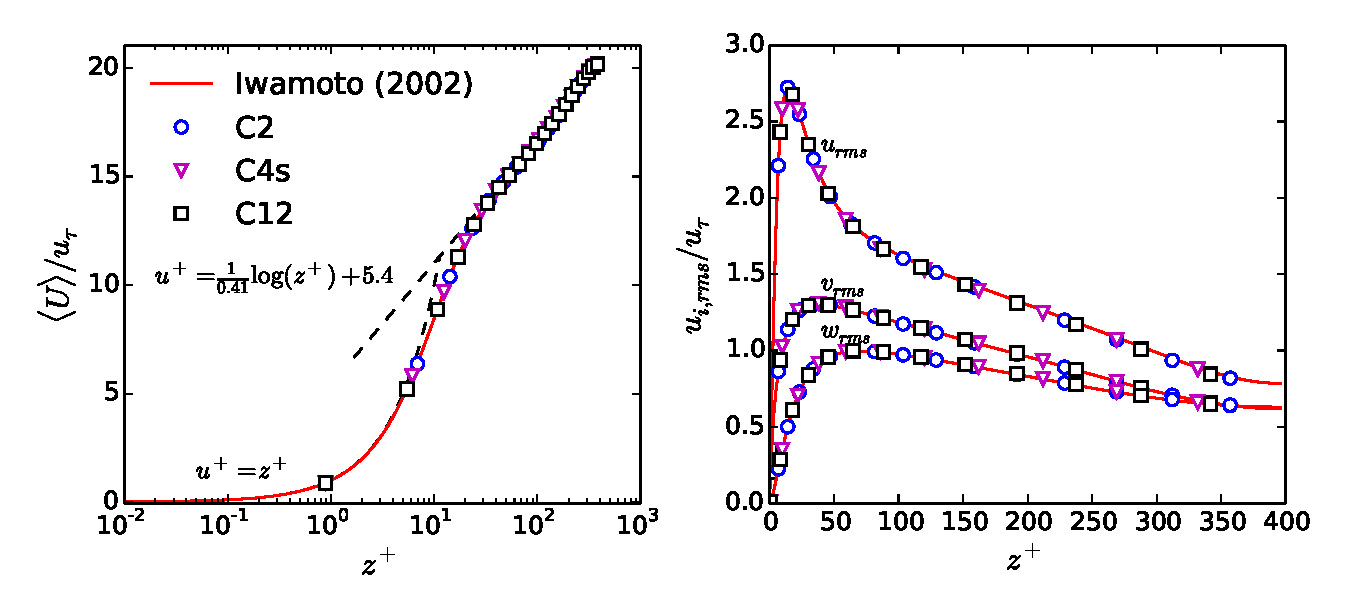
\includegraphics[width=\textwidth,trim= 0cm 0.35cm 0cm 0.3cm,clip]{chapters/turbulent_inflow/spbc/figure3}
			\caption{Comparison of C2, C4$s$ and C12 cases with reference data from \cite{iwamoto2002reynolds} Left: Mean streamwise velocity profile. Right: Mean root-mean-square velocity fluctuations. The amount of symbols has been altered for every case solely for clarity.}
			\label{fig:validation}
		\end{figure}
		
		Figure~\ref{fig:topviewCHANNEL} shows the plan views of partially time-averaged streamwise velocity fields at a distance $z/\delta = 0.05$ ($z^+ \approx 20$) from the lower wall for each of the channel-flow cases. Averaging times range from $Tu_*/\delta=10$ to $100$, and results are shown for $0\leq x \leq \pi\delta$. The figure illustrates that for the smaller domain cases, i.e. C2 and C4, the locking effect leads to significant banded variations in mean velocity profiles in the spanwise direction. For shorter averaging horizons (i.e. up until $T u_* / \delta = 20$), the partial averages of the longer cases, i.e. C6 and C12, appear very similar to those of the shorter ones. However, for time-averaging windows $Tu_*/\delta \ge 60$, the spanwise inhomogeneity disappears for the longer domains C6 and C12. Note that the longest time-averaging horizon shown in these plots ($Tu_*/\delta=100$) corresponds to approximately 280 flow-through times of the C2 domain. Finally, Figure~\ref{fig:topviewCHANNEL} demonstrates that the shifted cases (C2$s$ and C4$s$) exhibit the same behavior as the C6 and C12 cases, even though the streamwise domain length is significantly smaller. 
		
		\begin{figure}
			\centering
			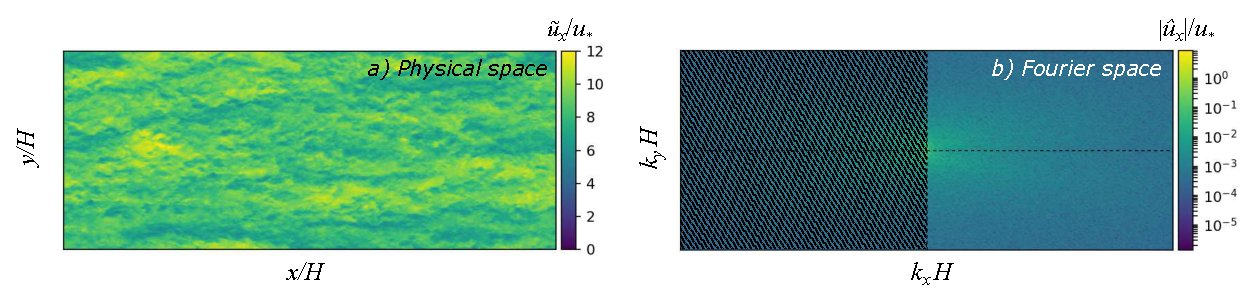
\includegraphics[width=\textwidth]{chapters/turbulent_inflow/spbc/figure4}
			\caption{Planview of time-averaged streamwise velocity in the buffer layer at a height of $z/\delta$ = 0.05 ($z^+ \approx 20$) from the lower wall for the C cases described in Table~\ref{tab:cases}. The illustrated domains are truncated in the streamwise direction at $x = \pi\delta$. Coloring is in units of $u/u_*$.}
			\label{fig:topviewCHANNEL}
		\end{figure}
		
		Figure~\ref{fig:delta_factorCHANNEL} provides a more quantitative illustration of the spanwise inhomogeneities in the simulation with the normalized peak-to-trough variation $\Delta$, defined as
		\begin{equation}
		\Delta(x,z,T) \equiv \frac{1}{\langle U \rangle (z,T)} \bigg [ \max_y \{ U(x,y,z,T) \} - \min_y \{ U(x,y,z,T)  \}  \bigg ],
		\end{equation}
		where U is the time-averaged streamwise velocity over a time window T, and $\langle \cdot \rangle$ denotes a horizontal averaging operation. Note that $\Delta(x,z,T)$ is virtually independent of the streamwise location $x$, hence we will implicitly refer to $\Delta(z,T)$ as the value at the inflow plane. Figure~\ref{fig:delta_factorCHANNEL}a shows $\Delta$ at $z/\delta = 0.05$, corresponding to the plan views in Figure~\ref{fig:topviewCHANNEL}. It confirms the statement from previous paragraph that, for shorter time windows up to $Tu_*/\delta = 20$, all non-shifted cases seem to have a similar $\Delta$. Longer time averaging decreases $\Delta$, up to a certain point around $Tu_*/\delta = 70$, after which asymptotic behavior is observed. Moreover, the shifted C4$s$ case closely resembles the behavior of the longer periodic C6 and C12 cases. The C2$s$ case finally also reaches the same asymptote as C4$s$, C6 and C12 for large $Tu_*/\delta$. Figure~\ref{fig:delta_factorCHANNEL}b illustrates the height-dependence of $\Delta$ for all cases for the longest time-horizon $Tu_*/\delta = 100$. As expected, spanwise variations are highest closer to the channel walls, where velocity fluctuations are strongest. This was also observed in \cite{fishpool2009persistent}.
		
		\begin{figure}
			\centering
			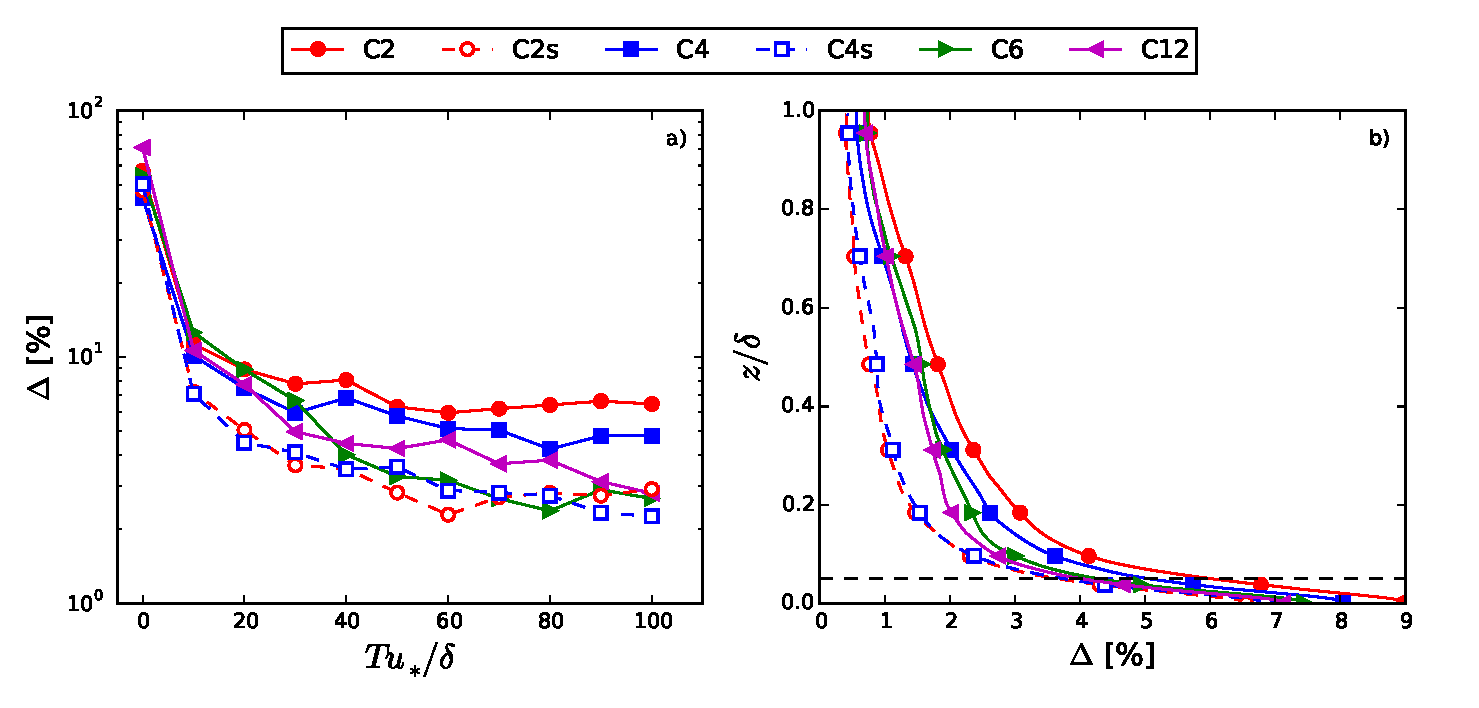
\includegraphics[width=\textwidth, trim= 0cm 0.15cm 0cm 0.cm,clip]{chapters/turbulent_inflow/spbc/figure5}
			\caption{Peak-to-trough spanwise inhomogeneity factor $\Delta$ for the channel flow DNS C cases: \emph{a)} $\Delta$ in function of time-averaging window $Tu_*/\delta$ (at height $z/\delta = 0.05$). \emph{b)} $\Delta$ in function of height $z/\delta$ (at final time-averaging window $Tu_*/\delta = 100$). The dashed line indicates $z/\delta = 0.05$. To increase statistical convergence of \emph{b)}, we averaged over both the streamwise direction and the 2 halves of the channel. }
			\label{fig:delta_factorCHANNEL}
		\end{figure}
		
		To conclude the discussion, Figure~\ref{fig:correlationsC} shows longitudinal autocorrelations of streamwise velocity $\rho_{uu}$.
		Since the non-shifted cases (i.e. C2, C4, C6 and C12) apply classical periodic boundary conditions, the autocorrelation of these
		simulations attain values of 1 at $r_x = L_x$ by definition. This is not the case for the shifted simulations C2$s$ and C4$s$. The
		autocorrelation of case C2 does not reach a zero value over its streamwise domain length, illustrating that the simulation domain is
		too short. Similarly, the autocorrelation of case C4 barely reaches a zero value at $r_x/\delta \approx 2 \pi$, before increasing to unity again. Both these observations show that the domains of C2 and C4 are too short to achieve full decorrelation over the streamwise domain length, explaining the banded structure in Figure~\ref{fig:topviewCHANNEL}, and the high $\Delta$-values in Figure~\ref{fig:delta_factorCHANNEL}. The longer cases C6 and C12 have an extended region of zero correlations. Both shifted cases, C2$s$ and C4$s$, also achieve decorrelation over their domain length. Moreover, note that C2$s$ and C4$s$ match virtually perfectly with the longer cases over their domain length, indicating that the shifting operation does not have any adverse effects on the longitudinal autocorrelation behavior.
		
		\begin{figure}
				\centering
			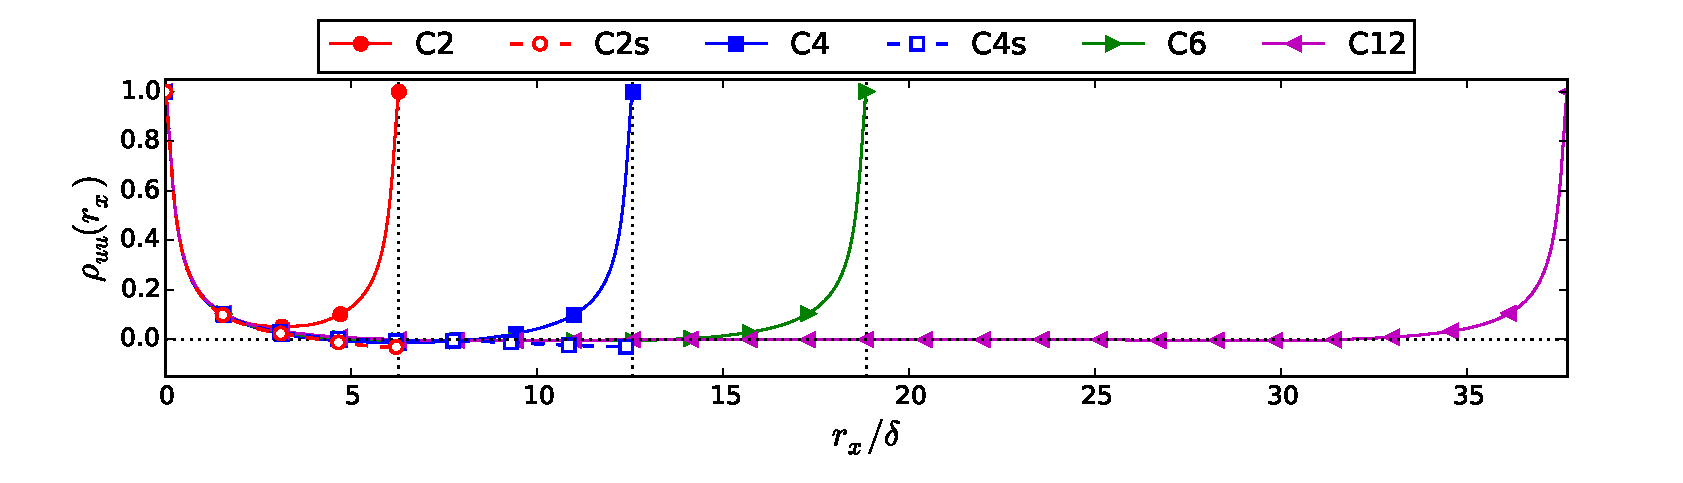
\includegraphics[width=\textwidth,trim= 0cm 0.2cm 0cm 0.cm,clip]{chapters/turbulent_inflow/spbc/figure6}
			\caption{One-dimensional longitudinal autocorrelations $\rho_{uu}(r_x)$ at $z/\delta = 0.05$ for the C cases. The vertical black dotted lines represent the domain lengths of the shorter cases, i.e. $L_x = 2\pi\delta$, $4\pi\delta$ and $6\pi\delta$, from left to right.}
			\label{fig:correlationsC}
		\end{figure}
		
		
		\subsubsection{Fully-developed high-Reynolds number half-channel flow}
		We now turn to the simulation results of the high Reynolds-number half-channel (HC) cases. Figure~\ref{fig:topviewHC} shows plan views of partially time-averaged streamwise velocity fields at a distance $z/\delta = 0.1$ from the surface. Firstly, note that the color range for the HC cases in this figure is significantly wider than for the C cases shown in Figure~\ref{fig:topviewCHANNEL}. For this much higher Reynolds number, it is observed that even the longest HC12 case is influenced by the spanwise locking of structures, though it should be noted that the effect is much smaller than for the HC1 and HC2 cases. This is not unexpected, as VLSM in high-Reynolds number boundary layers carry more kinetic energy and tend to be longer than those observed at low Reynolds numbers \citep{balakumar2007large,hutchins2007evidence,hutchins2007large}. For instance, structures of size $20\delta$ have been reported in LES of the atmospheric boundary layer \citep{fang2015large}.
		Looking at the results from the shifted periodic boundary condition cases HC2$s$ and HC4$s$ in Figure~\ref{fig:topviewHC}, it is seen that the spanwise inhomogeneities are reduced from the outset onwards, leading to results that are even more homogeneous than the HC12 case, even though domain lengths are significantly shorter. 
		
		% Topview of channel flows
		\begin{figure}
						\centering
			\includegraphics[width=\textwidth]{chapters/turbulent_inflow/spbc/figure7}
			\caption{Planview of time-averaged streamwise velocity in the log-law region at a height of $z/\delta$ = 0.1 ($z/z_0 = 10^3$) from the surface for the HC cases described in Table~\ref{tab:cases}. The illustrated domains are truncated in the streamwise direction at $x = \pi$. Coloring is in units of  $u/u_*$.}
			\label{fig:topviewHC}
		\end{figure}
		
		Figure~\ref{fig:delta_factorHC} illustrates the error $\Delta$ described above for the HC cases. Figure~\ref{fig:delta_factorHC}a again shows the dependency of $\Delta$ on the time-averaging window $Tu_*/\delta$ at a height $z/\delta = 0.1$, corresponding to the plan views in Figure~\ref{fig:topviewHC}. It can be seen that the shifted cases HC2$s$ and HC4$s$ show consistently lower inhomogeneities which, at the longest time-window $Tu_*/\delta = 60$, are approximately an order of magnitude lower than the non-shifted cases, the latter equaling roughly 10\% of the time-averaged mean velocity at the same height. Figure~\ref{fig:delta_factorHC}b illustrates the height dependence of $\Delta$ at the longest time-window. Generally, the highest $\Delta$-values can again be found closer to the wall (except for the very short HC1 case), although the reduction of $\Delta$ away from the wall is much lower than in the low Reynolds number case. 
		
		\begin{figure}
						\centering
			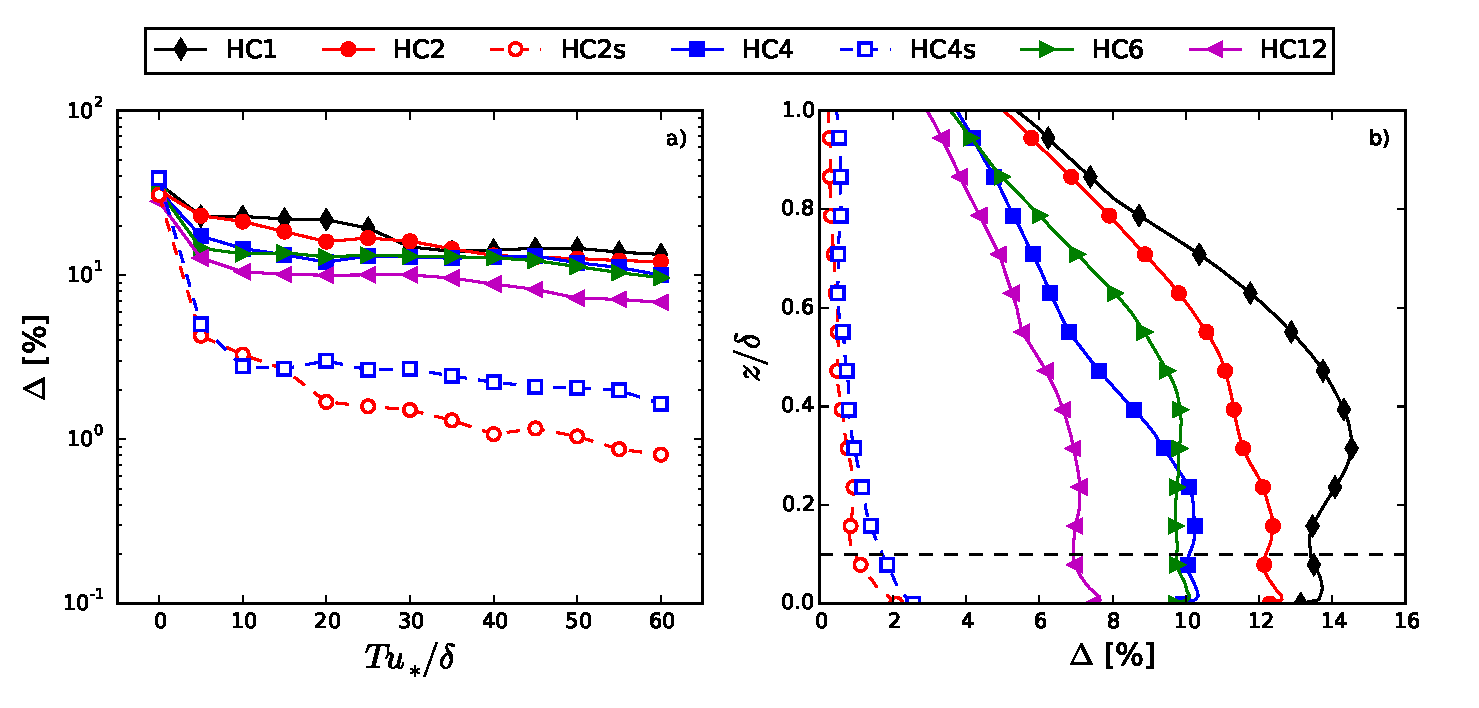
\includegraphics[width=\textwidth, trim= 0cm 0.15cm 0cm 0.cm,clip]{chapters/turbulent_inflow/spbc/figure8}
			\caption{Peak-to-trough spanwise inhomogeneity factor $\Delta$ for the half-channel flow LES HC cases: \emph{a)} $\Delta$ in function of time-averaging window $Tu_*/\delta$ (at height $z/\delta = 0.1$). \emph{b)} $\Delta$ in function of height $z/\delta$ (at final time-averaging window $Tu_*/\delta = 60$). The dashed line indicates $z/\delta = 0.1$.}
			\label{fig:delta_factorHC}
		\end{figure}
		
		Figure~\ref{fig:correlations} illustrates longitudinal autocorrelations $\rho_{uu}$ for each of the HC cases. Similar to the C cases
		from previous section, the non-shifted cases  are perfectly correlated at $r_x = L_x$ due to the periodic boundary conditions.
		Moreover, except for HC12, all conventionally periodic cases fail to achieve decorrelation of turbulent structures over their
		streamwise domain length (e.g. for the HC2 case with a conventional domain length $L_x = 2\pi\delta$,  $\rho_{uu}$ does not drop below
		0.2), which suggests the presence and persistence of domain-scale coherent structures. Although HC12 reaches $\rho_{uu} = 0$ at
		$r_x/\delta = 6\pi$, this is not sufficient to avoid the locking effect, as was also observed in case C4 of the previous section. The
		shifted cases HC2$s$ and HC4$s$ however  clearly show decorrelation between the inlet and outlet of the domain. The negative values of
		$\rho_{uu}$ at $r_x = L_x$ can be attributed to a combination of a spanwise shift length $d_s = 0.5 \delta$ and the negatively
		correlated counter-rotating vortices neighboring the VLSM in the spanwise direction \citep{tomkins2003spanwise, hutchins2012towards} ,
		transversal correlations omitted here for brevity. Finally, note that the HC4$s$ case achieves a zero-crossing of $\rho_{uu}$ at
		$r_x/\delta \approx 10$.  This is consistent with the results obtained by \cite{fang2015large} who performed a very similar case on a
		much larger periodic domain ($L_x = 32\pi\delta$, $L_y = 4\pi\delta$). This suggests that a simulation domain with streamwise length $L_x = 4\pi\delta$, combined with shifted periodic boundary conditions, produces coherent turbulent structures with the same autocorrelation behavior as the ones observed in much larger domains. 
		
		\begin{figure}
						\centering
			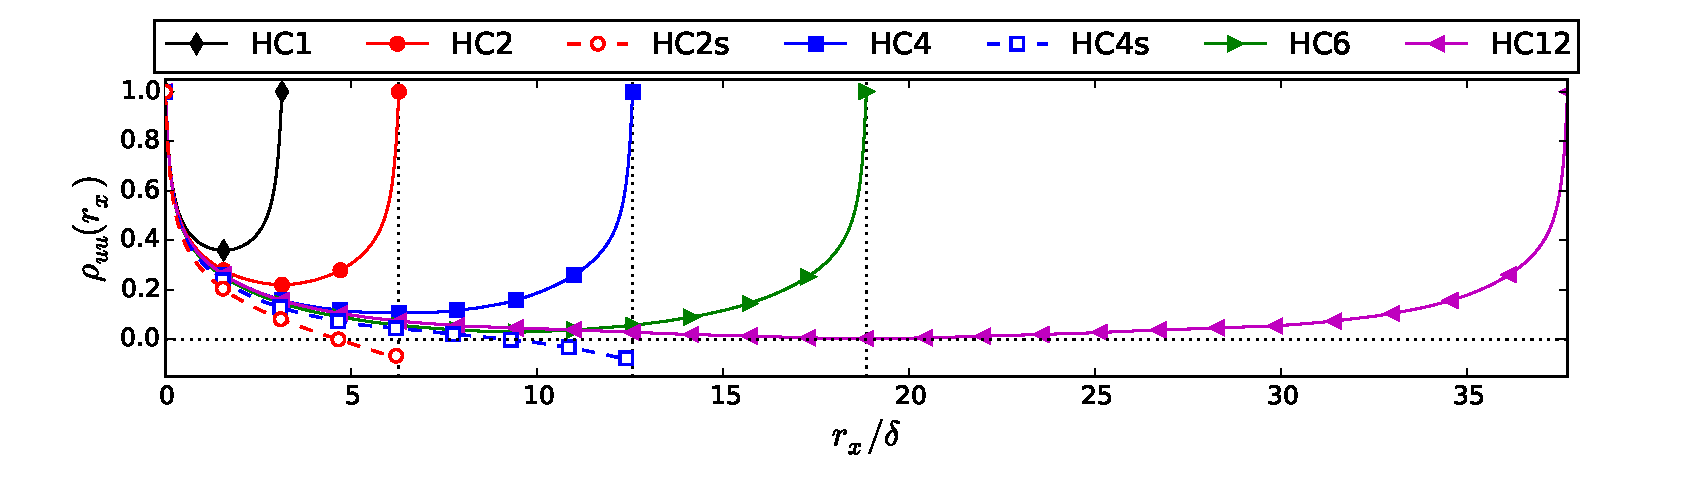
\includegraphics[width=\textwidth,trim= 0cm 0.2cm 0cm 0.cm,clip]{chapters/turbulent_inflow/spbc/figure9}
			\caption{One-dimensional longitudinal autocorrelations $\rho_{uu}(r_x)$ at $z/\delta = 0.1$ for the HC cases. The vertical black dotted lines represent the domain lengths of the shorter cases, i.e. $L_x = \pi$, $2\pi$, $4\pi$ and $6\pi$, from left to right.}
			\label{fig:correlations}
		\end{figure}
		
		Finally, we present the method's dependency on the user-defined shifting distance $d_s$ in Figure~\ref{fig:ds_dependency}. Here, we show the spanwise profiles of time-averaged streamwise velocity component for the cases HC2$s$ and HC2 defined above, as well as four additional shifted cases simulated on the HC2$s$ domain with a range of $d_s$ values. Profiles are illustrated at a height $z/\delta = 0.1$ for a time-averaging window $Tu_*/\delta = 20$. The figure illustrates that satisfactory results are also obtained for $d_s = \delta/4$, $\delta$, and $d_s = 3\delta/2$. For completeness, we include a case with $d_s = L_y/2$ as an example of a poor choice of shifting distance. It is observed that, for the latter case, inhomogeneities are replicated to multiple spanwise locations while they are only marginally attenuated.
		
		\begin{figure}[t]
						\centering
			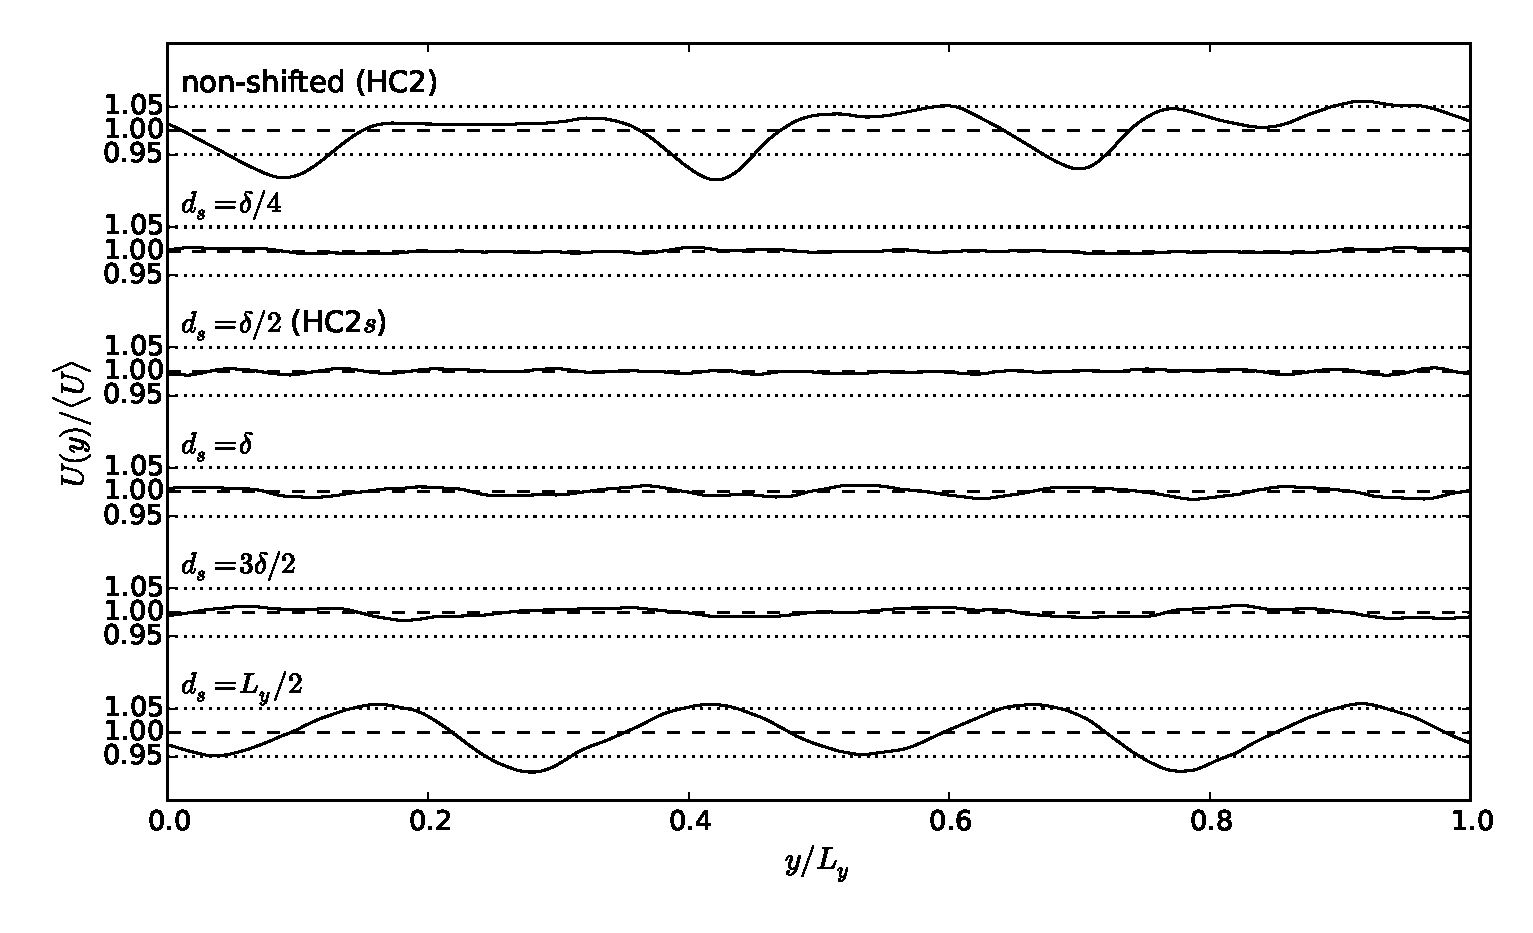
\includegraphics[width=\textwidth,, trim = 0 10 0 10,clip]{chapters/turbulent_inflow/spbc/figure10}
			\caption{Time-averaged streamwise velocity component at $z/\delta = 0.1$ as a function of spanwise location for various shifting distances $d_s$. Profiles are averaged over the streamwise direction and normalized by their horizontally-averaged values. Time averages calculated for a window of $Tu_*/\delta = 20$.}
			\label{fig:ds_dependency}
		\end{figure}
		
		
	\subsection{Application to a spatially developing wind-farm boundary layer}\label{sec:inflow_shifted_demo}
	As shown in previous paragraph, shifted periodic boundary conditions can effectively reduce spanwise variations of physically spanwise-homogeneous flows that are simulated on relatively short domains. We conclude the discussion on shifted periodic boundary conditions with an application case of ABL flow through a wind farm. The HC2, HC4, HC4$s$, HC6, and HC12 cases defined above are used as precursor simulations, providing inflow conditions to a main simulation domain with dimensions $L_x \times L_y \times H = 1.5\pi \delta \times 2\pi \delta \times \delta$. The wind farm consists of a $4 \times 12$ array of turbines with hub height $z_h/\delta = 0.10$, diameter $D/\delta = 0.10$ and steady thrust coefficient $\widehat{C}_T' = 4/3$ (see Figure~\ref{fig:WF}a). The grid resolution and turbine spacing ($S_x = 7.85D$, $S_x/S_y = 1.5$) correspond to the well-established A1 base case from \cite{calaf2010large}. In the following discussion, a column (row) is defined as a set of turbines located at the same spanwise (streamwise) coordinate.
	Simulation results are shown in Figure~\ref{fig:WF}. The simulations were performed for a time horizon of $Tu_*/\delta = 15$, corresponding to a physical time of slightly over 8 hours for typical atmospheric conditions ($u_* = 0.5$ m s$^{-1}$, $\delta = 1000$ m). Figure~\ref{fig:WF}a shows time-averaged contours of streamwise velocity at hub height, using the HC2 case as inflow generator. As shown in the figure, the spanwise locking effect of streamwise-elongated structures leads to an unrealistic distribution of high and low velocity regions among the different turbine columns in the wind farm, which in turn causes the large differences in power extraction between columns, as shown in Figure~\ref{fig:WF}b. As further observed in Figures~\ref{fig:WF}c and~\ref{fig:WF}d, when employing a shifted periodic boundary condition in the precursor domain (i.e. HC4$s$) this spanwise inhomogeneity in averages disappears over long time averages. 
	
	\begin{figure}
		\centering
		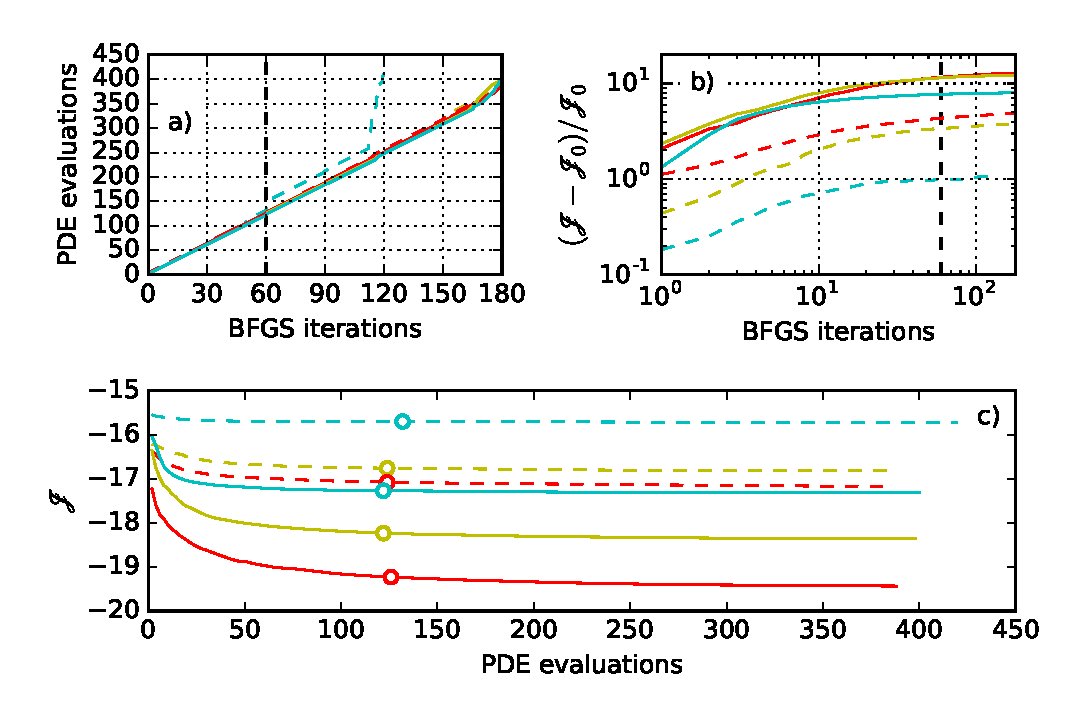
\includegraphics[width=0.9\textwidth]{chapters/turbulent_inflow/spbc/figure11}
		\caption{Wind-farm demo cases. \emph{a)} \& \emph{c)}: Planview of time-averaged flow field using HC2 (\emph{a}) and HC4$s$ (\emph{c}) as inflow simulation. \emph{b)} \& \emph{d)}: Time-averaged turbine power for different columns for non-shifted cases (\emph{b}), and shifted HC4$s$ case (\emph{d}). Powers are normalized by farm-averaged power (dashed black lines). Cases are shifted vertically for clarity. Dotted black lines indicate deviations of $\pm$10\% from the farm average.}
		\label{fig:WF}
	\end{figure}
	
	
	\subsection{Interim summary}
	The shifted periodic boundary conditions described in this section provide a simple yet efficient method to avoid the persistent spanwise locking of large-scale turbulent flow structures in canonical wall-bounded flow simulations with periodic lateral boundary conditions. The shifted periodic boundary condition approach replaces the streamwise periodicity by a spanwise shifted one, hence distributing turbulent structures amongst spanwise locations. The method is effective in obtaining better spanwise convergence of time-averaged flow fields for various flow cases and simulation strategies, as illustrated by a suite of low Reynolds number channel flows using direct numerical simulation and very high Reynolds number half-channel flows using large-eddy simulation. A wind-farm demonstration case showed one of many possible practical applications in which the method is useful.

	
\section{Summary}\label{sec:inflow_summary}
The current chapter has addressed the issue of generating unsteady and coherent turbulent inflow conditions for turbulence-resolving simulations of spatially developing flows in the context of wind-farm LES used by the optimal control studies in later chapters. A literature review uncovered the dichotomy between synthetic and Navier--Stokes based precursor inflow methods, and a comparative study between both indicated the better quality of the latter, especially when mechanisms such as wake meandering and turbulent entrainment are to be resolved properly. The precursor method implementation in the SP--Wind framework was elaborated, capable of an online concurrent mode and an offline database mode. Thereafter, a generalization of concurrent precursor methods to time-varying mean-flow directions was presented and illustrated based upon a LES study of the Horns Rev wind farm. Subsequently, shifted periodic boundary conditions were presented to alleviate the spanwise locking effect associated with periodic boundary conditions on relatively short streamwise domains. Furthermore, the application of these boundary conditions in a precursor simulation for a spatially developing wind-farm LES was shown. 

%%%%%%%%%%%%%%%%%%%%%%%%%%%%%%%%%%%%%%%%%%%%%%%%%%
% Keep the following \cleardoublepage at the end of this file, 
% otherwise \includeonly includes empty pages.
\cleardoublepage
